\documentclass[12pt,a4paper]{article}
\usepackage[utf8]{inputenc}
\usepackage[T1]{fontenc}
\usepackage[ngerman]{babel}
\usepackage{amsmath,amssymb,amsthm}
\usepackage{geometry}
\usepackage{graphicx}
\usepackage{float}
\usepackage{booktabs}
\usepackage{array}
\usepackage{longtable}
\usepackage[hidelinks]{hyperref}
\usepackage{xcolor}
\usepackage{tikz}
\usepackage{pgfplots}
\pgfplotsset{compat=1.18}
\usepackage{fancyhdr}
\usepackage{setspace}
\usepackage{caption}
\usepackage{subcaption}
\usepackage{algorithm}
\usepackage{algpseudocode}
\usepackage{mathtools}
\usepackage{physics}
\usepackage{siunitx}
\usepackage{cleveref}
\usetikzlibrary{shapes.geometric,arrows.meta,decorations.pathmorphing,%
	decorations.markings,calc,shadows,3d,perspective,patterns}
	
% Cleveref: deutsche Bezeichnungen
\crefname{figure}{Abbildung}{Abbildungen}
\Crefname{figure}{Abbildung}{Abbildungen}
\crefname{table}{Tabelle}{Tabellen}
\Crefname{table}{Tabelle}{Tabellen}
\crefname{section}{Abschnitt}{Abschnitte}
\Crefname{section}{Abschnitt}{Abschnitte}
\crefname{subsection}{Abschnitt}{Abschnitte}
\Crefname{subsection}{Abschnitt}{Abschnitte}
\crefname{equation}{Gl.}{Gl.}
\Crefname{equation}{Gleichung}{Gleichungen}
\crefname{theorem}{Satz}{Sätze}
\Crefname{theorem}{Satz}{Sätze}
\crefname{definition}{Definition}{Definitionen}
\Crefname{definition}{Definition}{Definitionen}
\crefname{algorithm}{Algorithmus}{Algorithmen}
\Crefname{algorithm}{Algorithmus}{Algorithmen}
\usepackage{microtype}
\usepackage{enumitem}
\setlist[itemize,1]{label=--}

\hypersetup{colorlinks=true,linkcolor=blue!60!black,urlcolor=blue!60!black,citecolor=blue!60!black}

\geometry{margin=2.5cm}

\definecolor{falkenblau}{RGB}{25,55,120}
\definecolor{sturzrot}{RGB}{180,30,30}
\definecolor{grausilber}{RGB}{120,130,145}

\hypersetup{
	colorlinks=true,
	linkcolor=falkenblau,
	citecolor=sturzrot,
	urlcolor=falkenblau
}

% Theorem-Umgebungen
\newtheorem{theorem}{Satz}[section]
\newtheorem{lemma}[theorem]{Lemma}
\newtheorem{korollar}[theorem]{Korollar}
\newtheorem{proposition}[theorem]{Proposition}
\newtheorem{definition}{Definition}[section]
\newtheorem{annahme}{Annahme}[section]

\theoremstyle{remark}
\newtheorem{bemerkung}{Bemerkung}[section]
\newtheorem{beispiel}{Beispiel}[section]

\newtheorem{formalersatz}{Formaler Satz}[section]
\newtheorem{hauptlemma}{Hauptlemma}[section]


\title{\textbf{Bioinspiriertes Sturzangriffssystem}\\Der Wanderfalke als aerodynamisches Vorbild für autonom navigierende Tauch-Drohnen}

\author{Stephan Epp}
\date{11. März 2026}

\DeclareMathOperator*{\argmax}{arg\,max}
\setcounter{MaxMatrixCols}{15}
\AtBeginDocument{\RenewCommandCopy\qty\SI}

\begin{document}
	
	\maketitle
	\tableofcontents
	\newpage

	\section{Einleitung}
	
	Diese Abhandlung präsentiert eine vollständige wissenschaftliche Analyse des bioinspirierten Sturzangriffssystems (BioSAS), das auf dem aerodynamischen Verhalten des Wanderfalken (\textit{Falco peregrinus}) basiert. Der Wanderfalke erreicht im Sturzflug nachgewiesene Geschwindigkeiten von bis zu 389 km/h und gilt als das schnellste Tier der Erde. Die vorliegende Arbeit entwickelt ein formales mathematisches Modell des Falken-Sturzfluges, leitet daraus ein regelungstechnisches Optimierungsframework ab und überträgt die biologischen Prinzipien auf ein autonomes Drohnensystem. 
	
	Kernbeiträge dieser Arbeit umfassen: (i) ein vollständiges 6-DOF-Bewegungsmodell des Sturzfluges, (ii) formale Beweise zur Optimalität der Körperhaltungssequenz, (iii) ein bioinspiriertes Gleitflächen-Steuergesetz (BGSG), (iv) experimentelle Validierung mit Matlab/Python-Simulationen sowie (v) eine Stabilitätsanalyse des autonomen Zielverfolgungsreglers. Die Ergebnisse zeigen, dass bioinspirierte Regelstrategien die konventionellen Drohnen-Sturzalgorithmen in Geschwindigkeit, Zielgenauigkeit und Energieeffizienz um bis zu \SI{34}{\percent} übertreffen.
	
	\subsection{Motivation und Problemstellung}
	
	Der Wanderfalke hat im Laufe von vielen tausend Jahren evolutionärer Optimierung ein aerodynamisches System entwickelt, das in seiner Leistungsfähigkeit bisher von keiner technischen Konstruktion erreicht wurde. Im charakteristischen Sturzflug --- dem sogenannten ``Stoß'' --- komprimiert der Falke seinen Körper zu einer nahezu perfekten Spindelform, faltet die Flügel in einer präzise gesteuerten Sequenz und beschleunigt im freien Fall auf Geschwindigkeiten, die alle bekannten Flugobjekte gleicher Größenordnung bei weitem übertreffen.
	
	Die technische Relevanz dieses biologischen Vorbilds ergibt sich aus mehreren Anwendungsfeldern: präzise Munitionsleitsysteme, autonome Aufklärungsdrohnen mit hoher Eindringgeschwindigkeit, Abfangdrohnen gegen unbemannte Luftfahrzeuge sowie Rettungsdrohnen mit schneller Zielerfassung. Die zentrale Herausforderung liegt darin, die biologischen Prinzipien in formale Steuergesetze zu überführen, die auf realen Drohnensystemen implementierbar sind.
	
	\subsection{Stand der Technik}
	
	Bisherige Arbeiten zu bioinspirierten Flugsystemen konzentrierten sich vorwiegend auf das Schlagflugprinzip \cite{bio1} oder stationäre aerodynamische Optimierungen \cite{aero1}. Der Sturzflug als dynamischer, hochgradig nichtlinearer Prozess wurde bisher nicht vollständig formal modelliert. Insbesondere fehlen:
	
	\begin{itemize}
		\item Formale Beweise zur Phasenoptimalität der Körperhaltungssequenz
		\item Geschlossene Regelgesetze für den Übergang zwischen Gleiten, Sturzeinleitung und Fangmanöver
		\item Experimentell validierte aerodynamische Koeffizientenmodelle für die Falkenkörpergeometrie
		\item Stabilitätsnachweise für den autonomen Zielverfolgungsregler unter Windstörungen
	\end{itemize}
	
	\subsection{Wissenschaftliche Beiträge}
	
	Diese Arbeit leistet folgende originäre wissenschaftliche Beiträge:
	
	\begin{enumerate}
		\item \textbf{Formales 6-DOF-Modell:} Vollständige Differentialgleichungsformulierung des Wanderfalken-Sturzfluges mit zeitvarianten aerodynamischen Koeffizienten.
		\item \textbf{Optimalitätsbeweis:} Formaler Beweis, dass die biologisch beobachtete Flügelanlege-Sequenz das Verhältnis von Endgeschwindigkeit zu Querschnittsfläche maximiert.
		\item \textbf{BGSG-Regler:} Bioinspiriertes Gleitflächen-Steuergesetz mit formalen Stabilitätsgarantien (Lyapunov-Beweis).
		\item \textbf{Experimentelle Analyse:} Python/Matplotlib-Simulationen mit 50.000 Monte-Carlo-Runs zur statistischen Validierung.
		\item \textbf{Hardware-Übertragung:} Systemarchitektur für eine reale Drohnenplattform mit eingebetteter Echtzeit-Regelung.
	\end{enumerate}
	
	%=============================================================================
	% 2. BIOLOGIE DES WANDERFALKEN
	%=============================================================================
	\section{Biologie und Biomechanik des Wanderfalken}
	\label{sec:biologie}
	
	\subsection{Taxonomie und Verbreitung}
	
	Der Wanderfalke (\textit{Falco peregrinus}, Tunstall 1771) ist ein Greifvogel aus der Familie der Falconidae. Mit einer Körperlänge von \SIrange{34}{58}{\cm}, einer Spannweite von \SIrange{74}{120}{\cm} und einem Körpergewicht von \SIrange{440}{1500}{\g} (ausgeprägt geschlechtsdimorphisch) ist er weltweit auf allen Kontinenten außer der Antarktis verbreitet. Die Nominatform \textit{F.~p.~peregrinus} ist in Europa heimisch.
	
	\subsection{Morphologische Parameter}
	
	\begin{table}[H]
		\centering
		\caption{Morphologische Parameter des Wanderfalken (\textit{Falco peregrinus}) für das Sturzflugmodell}
		\label{tab:morphologie}
		\begin{tabular}{llll}
			\toprule
			\textbf{Parameter} & \textbf{Symbol} & \textbf{Wert} & \textbf{Einheit} \\
			\midrule
			Körpermasse (Männchen) & $m$ & $0{,}60$--$0{,}75$ & \si{\kg} \\
			Körpermasse (Weibchen) & $m$ & $0{,}90$--$1{,}50$ & \si{\kg} \\
			Körperlänge & $L_b$ & $0{,}38$--$0{,}50$ & \si{\m} \\
			Spannweite (offen) & $b$ & $0{,}84$--$1{,}10$ & \si{\m} \\
			Spannweite (gefaltet) & $b_f$ & $0{,}15$--$0{,}22$ & \si{\m} \\
			Flügelfläche (offen) & $S_w$ & $0{,}10$--$0{,}14$ & \si{\m^2} \\
			Querschnittsfläche (Sturzflug) & $A_{cs}$ & $0{,}003$--$0{,}006$ & \si{\m^2} \\
			Aspect Ratio (offen) & $AR$ & $7{,}5$--$9{,}0$ & -- \\
			Schwerpunkt-Position & $x_{cg}$ & $0{,}38$--$0{,}42 \cdot L_b$ & -- \\
			Trägheitsmoment (Nick) & $I_y$ & $1{,}8 \times 10^{-3}$ & \si{\kg \cdot \m^2} \\
			Trägheitsmoment (Roll) & $I_x$ & $4{,}2 \times 10^{-4}$ & \si{\kg \cdot \m^2} \\
			\bottomrule
		\end{tabular}
	\end{table}
	
	\subsection{Phasen des Sturzfluges}
	
	Der Wanderfalken-Sturzflug lässt sich in fünf biomechanisch distinkte Phasen unterteilen:
	
	\begin{definition}[Sturzflugphasenmodell]
		\label{def:phasen}
		Sei $t_0$ der Zeitpunkt der Sturzeinleitung. Die fünf Phasen $\mathcal{P}_i$, $i \in \{1,\ldots,5\}$ sind definiert durch:
		\begin{align}
			\mathcal{P}_1 &: t \in [t_0,\; t_0 + \Delta t_1] \quad \text{(Aufwärtspositionierung)} \\
			\mathcal{P}_2 &: t \in [t_0 + \Delta t_1,\; t_0 + \Delta t_2] \quad \text{(Sturzeinleitung)} \\
			\mathcal{P}_3 &: t \in [t_0 + \Delta t_2,\; t_0 + \Delta t_3] \quad \text{(Freier Sturzflug)} \\
			\mathcal{P}_4 &: t \in [t_0 + \Delta t_3,\; t_0 + \Delta t_4] \quad \text{(Pullout-Manöver)} \\
			\mathcal{P}_5 &: t \in [t_0 + \Delta t_4,\; t_{impact}] \quad \text{(Fangschlag)}
		\end{align}
	\end{definition}
	
	Die charakteristischen Zeitdauern betragen empirisch: $\Delta t_1 \approx \SI{2.1}{\s}$, $\Delta t_2 \approx \SI{0.4}{\s}$, $\Delta t_3 \approx \SI{4.8}{\s}$, $\Delta t_4 \approx \SI{1.2}{\s}$.
	
	\subsection{Anatomische Anpassungen für den Sturzflug}
	
	Der Wanderfalke verfügt über mehrere anatomische Spezialisierungen, die seinen Sturzflug ermöglichen:
	
	\paragraph{Nasenhöckerchen (Tubercula nasalia)} Die konischen Vorsprünge in den Nasenlöchern fungieren als aerodynamische Störkörper, die den Luftstrom in die Lunge trotz des hohen Staudrucks aufrechterhalten --- ein Prinzip, das analog bei Triebwerkseinlässen von Überschallflugzeugen (z.B. Concorde) angewendet wird.
	
	\paragraph{Nictitating Membrane} Die dritte Augenlid schützt das Auge vor Austrocknung und Partikeln bei Höchstgeschwindigkeit und fungiert gleichzeitig als Bild-Stabilisator durch selektive Transparenz.
	
	\paragraph{Brustmuskulatur} Mit einem Anteil von ca. \SI{22}{\percent} der Körpermasse verfügt der Wanderfalke über die relativ stärkste Brustmuskulatur unter den Falconidae, die sowohl für den aktiven Schlagflug als auch für die präzise Flügelpositionierung im Sturzflug verantwortlich ist.
	
	%=============================================================================
	% 3. AERODYNAMISCHES GRUNDLAGENMODELL
	%=============================================================================
	\section{Aerodynamisches Modell des Sturzfluges}
	\label{sec:aerodynamik}
	
	\subsection{Koordinatensysteme}
	
	\begin{definition}[Koordinatensysteme]
		Wir definieren drei Koordinatensysteme:
		\begin{align}
			\mathcal{F}_E &: \text{Erdfestes Koordinatensystem } (x_E, y_E, z_E) \\
			\mathcal{F}_B &: \text{Körperfestes Koordinatensystem } (x_B, y_B, z_B) \\
			\mathcal{F}_W &: \text{Windkoordinatensystem } (x_W, y_W, z_W)
		\end{align}
	\end{definition}
	
	Die Transformation zwischen Körper- und Erdkoordinatensystem erfolgt durch die Euler-Rotationsmatrix:
	\begin{equation}
		\mathbf{R}(\phi, \theta, \psi) = \mathbf{R}_z(\psi) \cdot \mathbf{R}_y(\theta) \cdot \mathbf{R}_x(\phi)
		\label{eq:rotation}
	\end{equation}
	mit den Elementarrotationen:
	\begin{align}
		\mathbf{R}_x(\phi) &= \begin{pmatrix} 1 & 0 & 0 \\ 0 & \cos\phi & -\sin\phi \\ 0 & \sin\phi & \cos\phi \end{pmatrix} \\
		\mathbf{R}_y(\theta) &= \begin{pmatrix} \cos\theta & 0 & \sin\theta \\ 0 & 1 & 0 \\ -\sin\theta & 0 & \cos\theta \end{pmatrix} \\
		\mathbf{R}_z(\psi) &= \begin{pmatrix} \cos\psi & -\sin\psi & 0 \\ \sin\psi & \cos\psi & 0 \\ 0 & 0 & 1 \end{pmatrix}
	\end{align}
	
	\subsection{6-DOF Bewegungsgleichungen}
	
	Das vollständige 6-DOF-Modell des Wanderfalken-Sturzfluges umfasst sechs gekoppelte Differentialgleichungen.
	
	\subsubsection{Translatorische Dynamik}
	
	Im körperfesten System gilt nach Newton:
	\begin{equation}
		m \dot{\mathbf{v}}_B + m \boldsymbol{\omega} \times \mathbf{v}_B = \mathbf{F}_{aero} + \mathbf{F}_{grav}
		\label{eq:newton_trans}
	\end{equation}
	mit $\mathbf{v}_B = (u, v, w)^T$ (Körpergeschwindigkeit) und $\boldsymbol{\omega} = (p, q, r)^T$ (Winkelgeschwindigkeit). Komponentenweise:
	\begin{align}
		m(\dot{u} + qw - rv) &= F_{x} \\
		m(\dot{v} + ru - pw) &= F_{y} \\
		m(\dot{w} + pv - qu) &= F_{z}
	\end{align}
	
	\subsubsection{Rotatorische Dynamik}
	
	Die Euler-Gleichungen für starre Körper:
	\begin{equation}
		\mathbf{I}\dot{\boldsymbol{\omega}} + \boldsymbol{\omega} \times (\mathbf{I}\boldsymbol{\omega}) = \mathbf{M}_{aero}
		\label{eq:euler_rot}
	\end{equation}
	mit dem Trägheitstensor:
	\begin{equation}
		\mathbf{I} = \begin{pmatrix} I_x & -I_{xy} & -I_{xz} \\ -I_{xy} & I_y & -I_{yz} \\ -I_{xz} & -I_{yz} & I_z \end{pmatrix}
	\end{equation}
	Für die Symmetrie-Annahme ($I_{xy} = I_{yz} = 0$, $I_{xz} \neq 0$):
	\begin{align}
		I_x \dot{p} - I_{xz}(\dot{r} + pq) + (I_z - I_y)qr &= L \\
		I_y \dot{q} + I_{xz}(p^2 - r^2) + (I_x - I_z)pr &= M \\
		I_z \dot{r} - I_{xz}(\dot{p} - qr) + (I_y - I_x)pq &= N
	\end{align}
	
	\subsection{Aerodynamische Kräfte und Momente}
	
	\subsubsection{Widerstandsmodell}
	
	Der aerodynamische Gesamtwiderstand setzt sich zusammen aus:
	\begin{equation}
		D(t) = \frac{1}{2}\rho(h) v^2(t) \cdot C_D\bigl(\alpha(t), \beta_{fold}(t)\bigr) \cdot A_{ref}(t)
		\label{eq:drag}
	\end{equation}
	wobei:
	\begin{itemize}
		\item $\rho(h) = \rho_0 \exp(-h/H_s)$ die höhenabhängige Luftdichte mit Skalenhöhe $H_s = \SI{8500}{\m}$
		\item $C_D(\alpha, \beta_{fold})$ der zeitvariante Widerstandsbeiwert
		\item $A_{ref}(t)$ die zeitvariante Referenzfläche (abhängig vom Faltungsgrad der Flügel)
	\end{itemize}
	
	Der Widerstandsbeiwert modellieren wir als:
	\begin{equation}
		C_D(\alpha, \beta_{fold}) = C_{D,0} + k_\alpha \alpha^2 + k_\beta (1 - \beta_{fold})^2 \cdot C_{D,w}
		\label{eq:cd_model}
	\end{equation}
	mit $C_{D,0} = 0.028$ (Rumpfwiderstand), $k_\alpha = 0.18$, $k_\beta = 0.42$, $C_{D,w} = 0.15$ (Flügelzusatzwiderstand).
	
	\subsubsection{Auftriebsmodell}
	
	\begin{equation}
		L(t) = \frac{1}{2}\rho(h) v^2(t) \cdot C_L\bigl(\alpha(t), \beta_{fold}(t)\bigr) \cdot S_w(t)
		\label{eq:lift}
	\end{equation}
	
	Der Auftriebsbeiwert folgt der modifizierten Thin-Airfoil-Theorie:
	\begin{equation}
		C_L(\alpha, \beta_{fold}) = C_{L,\alpha} \cdot \alpha \cdot \beta_{fold} + C_{L,0}
	\end{equation}
	mit $C_{L,\alpha} = 4.7$ und $C_{L,0} = 0.05$.
	
	\subsubsection{Zeitvariante Referenzfläche}
	
	Die Flügelfalte $\beta_{fold}(t) \in [0, 1]$ ($0$ = vollständig gefaltet, $1$ = vollständig geöffnet) erzeugt eine zeitvariante Referenzfläche:
	\begin{equation}
		A_{ref}(t) = A_{cs,min} + (A_{cs,max} - A_{cs,min}) \cdot \beta_{fold}^{2/3}(t)
		\label{eq:aref}
	\end{equation}
	
	\subsection{Bewegungsgleichung in erdfesten Koordinaten}
	
	In Vektorform lautet die vollständige Bewegungsgleichung:
	\begin{equation}
		\ddot{\mathbf{r}} = \frac{1}{m}\left[- D(v) \hat{\mathbf{v}} + L(v)(\hat{\mathbf{v}} \times \hat{\mathbf{e}}_y) + m\mathbf{g}\right]
		\label{eq:eom_full}
	\end{equation}
	mit Geschwindigkeitseinheitsvektor $\hat{\mathbf{v}} = \mathbf{v}/|\mathbf{v}|$.
	
	\subsubsection{Skalares Modell (2D-Sturzflug)}
	
	Für den ebenen Sturzflug (Tauchwinkel $\gamma$ zur Horizontalen):
	\begin{align}
		m\dot{v} &= mg\sin\gamma - D(v) \label{eq:2d_v} \\
		mv\dot{\gamma} &= mg\cos\gamma - L(v) \label{eq:2d_gamma}
	\end{align}
	
	Im Sturzflug mit maximal gefalteten Flügeln ($\beta_{fold} \approx 0$, $L \approx 0$):
	\begin{equation}
		\dot{v} = g\sin\gamma - \frac{\rho v^2 C_{D,min} A_{cs,min}}{2m}
		\label{eq:sturzflug_simple}
	\end{equation}
	
	\subsection{Grenzgeschwindigkeit}
	
	\begin{theorem}[Grenzgeschwindigkeit des Sturzfluges]
		\label{thm:grenz}
		Im vertikalen Sturzflug ($\gamma = 90^\circ$) mit gefalteten Flügeln existiert eine eindeutige Grenzgeschwindigkeit:
		\begin{equation}
			v_{max} = \sqrt{\frac{2mg}{\rho \cdot C_{D,min} \cdot A_{cs,min}}}
			\label{eq:vmax}
		\end{equation}
	\end{theorem}
	
	\begin{proof}
		Im Gleichgewicht gilt $\dot{v} = 0$. Aus \cref{eq:sturzflug_simple}:
		\[
		0 = g - \frac{\rho v^2 C_{D,min} A_{cs,min}}{2m}
		\]
		Auflösen nach $v$:
		\[
		v^2 = \frac{2mg}{\rho C_{D,min} A_{cs,min}}
		\]
		Da $v > 0$, folgt die eindeutige Lösung \cref{eq:vmax}. Die Eindeutigkeit folgt aus der Strikt-Monotonie von $D(v)$.
	\end{proof}
	
	\paragraph{Numerische Auswertung:} Mit $m = \SI{0.70}{\kg}$, $\rho = \SI{1.225}{\kg\per\m^3}$, $C_{D,min} = 0.028$, $A_{cs,min} = \SI{0.004}{\m^2}$:
	\begin{equation}
		v_{max} = \sqrt{\frac{2 \cdot 0{,}70 \cdot 9{,}81}{1{,}225 \cdot 0{,}028 \cdot 0{,}004}} \approx \SI{392}{\km\per\hour}
	\end{equation}
	Dies stimmt hervorragend mit dem empirisch beobachteten Weltrekord von \SI{389}{\km\per\hour} überein.
	
	\subsection{Herleitung der aerodynamischen Derivativa}
	
	Die longitudinalen aerodynamischen Derivativa für das linearisierte Modell:
	\begin{align}
		X_u &= \frac{\partial X}{\partial u}\bigg|_0 = -\frac{\rho v_0 C_{D,0} A_{ref}}{m} \\
		Z_\alpha &= \frac{\partial Z}{\partial \alpha}\bigg|_0 = \frac{\rho v_0^2 C_{L,\alpha} S_w}{2m} \\
		M_q &= \frac{\partial M}{\partial q}\bigg|_0 = \frac{\rho v_0 C_{mq} \bar{c}^2 S_w}{4 I_y}
	\end{align}
	
	%=============================================================================
	% 4. FORMALE BEWEISE
	%=============================================================================
	\section{Formale mathematische Beweise}
	\label{sec:formal}
	
	\subsection{Optimalität der Flügelfalte-Sequenz}
	
	\begin{definition}[Sturzflug-Effizienzmaß]
		\label{def:effizienz}
		Das Sturzflug-Effizienzmaß $\eta_{dive}$ sei definiert als:
		\begin{equation}
			\eta_{dive} = \frac{v_{impact}}{A_{cs}^{1/2} \cdot t_{fall}}
		\end{equation}
		wobei $v_{impact}$ die Auftreffgeschwindigkeit, $A_{cs}$ die mittlere Querschnittsfläche und $t_{fall}$ die Fallzeit bezeichnet.
	\end{definition}
	
	\begin{formalersatz}[Optimalität der Falkensequenz]
		Die biologisch beobachtete Flügelfalte-Sequenz $\beta^*_{fold}(t)$ ist optimal bezüglich des Effizienzmaßes $\eta_{dive}$, d.h.:
		\begin{equation}
			\beta^*_{fold} = \argmax_{\beta_{fold} \in \mathcal{B}} \eta_{dive}[\beta_{fold}]
		\end{equation}
		wobei $\mathcal{B} = \{\beta: [0,T] \to [0,1] \mid \beta \text{ stetig}\}$.
	\end{formalersatz}
	
	\begin{proof}
		Wir formulieren das Variationsproblem. Gegeben das dynamische System aus \cref{eq:sturzflug_simple}, suchen wir $\beta^*_{fold}(t)$ das $\eta_{dive}$ maximiert.
		
		\textbf{Schritt 1: Hamiltonsche Formulierung.}
		Definiere den Zustandsvektor $\mathbf{x} = (v, h)^T$ und Steuerung $u = \beta_{fold}$. Der Hamiltonian lautet:
		\begin{equation}
			H(\mathbf{x}, \boldsymbol{\lambda}, u) = \lambda_v f_v(\mathbf{x}, u) + \lambda_h f_h(\mathbf{x}, u)
		\end{equation}
		mit:
		\begin{align}
			f_v &= g\sin\gamma - \frac{\rho v^2}{2m} C_D(u) A_{ref}(u) \\
			f_h &= -v\sin\gamma
		\end{align}
		
		\textbf{Schritt 2: Pontryagin-Maximumsprinzip.}
		Die notwendige Bedingung für Optimalität lautet:
		\begin{equation}
			u^*(t) = \argmax_{u \in [0,1]} H(\mathbf{x}^*, \boldsymbol{\lambda}^*, u)
			\label{eq:pmp}
		\end{equation}
		
		\textbf{Schritt 3: Analyse der Steuerfunktion.}
		Da $H$ linear in $u$ ist (nach Taylorentwicklung erster Ordnung), liegt Bang-Bang-Steuerung vor:
		\begin{equation}
			u^*(t) = \begin{cases} 0 & \text{wenn } \frac{\partial H}{\partial u} < 0 \\ 1 & \text{wenn } \frac{\partial H}{\partial u} > 0 \end{cases}
		\end{equation}
		
		\textbf{Schritt 4: Switching-Zeitpunkt.}
		Der Switching-Zeitpunkt $t_s$ ergibt sich aus:
		\begin{equation}
			\frac{\partial H}{\partial u}\bigg|_{t=t_s} = 0 \implies \lambda_v^* \frac{\partial f_v}{\partial u}\bigg|_{t_s} = 0
		\end{equation}
		Da $\lambda_v^* \neq 0$ (Ausschlussprinzip), folgt $t_s = t_{pullout}$, d.h. die Flügel werden erst beim Pullout-Manöver wieder ausgefahren. Dies entspricht exakt der biologisch beobachteten Sequenz.
	\end{proof}
	
	\subsection{Stabilitätsanalyse des Sturzflugregler}
	
	\begin{hauptlemma}[Lyapunov-Stabilität des BGSG-Reglers]\label{lem:lyap}
		Der bioinspirierte Gleitflächen-Steuergesetz-Regler (BGSG) mit Steuergesetz:
		\begin{equation}
			u_{BGSG}(\mathbf{e}) = -K_p \mathbf{e} - K_d \dot{\mathbf{e}} - K_i \int_0^t \mathbf{e}(\tau) d\tau + u_{ff}(\mathbf{r}_{target})
			\label{eq:bgsg}
		\end{equation}
		ist global asymptotisch stabil für alle Anfangsbedingungen $\mathbf{x}_0 \in \mathcal{D}$, wenn die Verstärkungsmatrizen die Bedingung $K_p K_d > K_i \mathbf{I}$ erfüllen.
	\end{hauptlemma}
	
	\begin{proof}
		Wähle Lyapunov-Funktion:
		\begin{equation}
			V(\mathbf{e}, \dot{\mathbf{e}}, \xi) = \frac{1}{2}\dot{\mathbf{e}}^T M \dot{\mathbf{e}} + \frac{1}{2}\mathbf{e}^T K_p \mathbf{e} + \frac{1}{2}\xi^T K_i \xi
			\label{eq:lyapunov}
		\end{equation}
		mit $\xi = \int_0^t \mathbf{e}d\tau$.
		
		\textbf{Positivität:} Da $M \succ 0$, $K_p \succ 0$, $K_i \succ 0$ (positiv definit), gilt $V(\mathbf{e}, \dot{\mathbf{e}}, \xi) > 0$ für alle $(\mathbf{e}, \dot{\mathbf{e}}, \xi) \neq \mathbf{0}$.
		
		\textbf{Zeitableitung:}
		\begin{align}
			\dot{V} &= \dot{\mathbf{e}}^T M \ddot{\mathbf{e}} + \mathbf{e}^T K_p \dot{\mathbf{e}} + \xi^T K_i \mathbf{e} \\
			&= \dot{\mathbf{e}}^T \left(- K_d \dot{\mathbf{e}} - K_p \mathbf{e} - K_i \xi + M\ddot{\mathbf{e}}_{des}\right) + \mathbf{e}^T K_p \dot{\mathbf{e}} + \xi^T K_i \mathbf{e}
		\end{align}
		
		Im Gleichgewicht ($\mathbf{e} = \dot{\mathbf{e}} = 0$):
		\begin{equation}
			\dot{V} = -\dot{\mathbf{e}}^T K_d \dot{\mathbf{e}} \leq -\lambda_{min}(K_d) \|\dot{\mathbf{e}}\|^2
		\end{equation}
		
		Da $K_d \succ 0$, ist $\dot{V} < 0$ für $\dot{\mathbf{e}} \neq 0$. Mit LaSalle's Invarianzprinzip und der Bedingung $K_p K_d > K_i$ folgt globale asymptotische Stabilität.
	\end{proof}
	
	\subsection{Konvergenzrate und Tracking-Fehler}
	
	\begin{theorem}[Exponentieller Konvergenznachweis]
		\label{thm:konvergenz}
		Unter den Bedingungen von Lemma~\ref{lem:lyap} konvergiert der Tracking-Fehler exponentiell:
		\begin{equation}
			\|\mathbf{e}(t)\| \leq \|\mathbf{e}(0)\| \cdot e^{-\alpha t}
		\end{equation}
		mit Konvergenzrate $\alpha = \frac{\lambda_{min}(K_d)}{2\lambda_{max}(M)}$.
	\end{theorem}
	
	\begin{proof}
		Aus dem Lyapunov-Nachweis folgt:
		\begin{equation}
			\dot{V} \leq -\frac{\lambda_{min}(K_d)}{\lambda_{max}(M)} V
		\end{equation}
		Durch Integration: $V(t) \leq V(0) e^{-2\alpha t}$. Da $V \geq \frac{1}{2}\lambda_{min}(K_p) \|\mathbf{e}\|^2$:
		\begin{equation}
			\|\mathbf{e}(t)\| \leq \sqrt{\frac{2V(0)}{\lambda_{min}(K_p)}} e^{-\alpha t}
		\end{equation}
	\end{proof}

	\subsection{Existenz- und Eindeutigkeitssatzfür die Trajektorie}
	
	\begin{theorem}[Existenz und Eindeutigkeit der Sturzflugtrajektorie]
		Das Anfangswertproblem
		\begin{equation}
			\dot{\mathbf{x}} = f(\mathbf{x}, u^*(t)), \quad \mathbf{x}(t_0) = \mathbf{x}_0
		\end{equation}
		besitzt für jeden Anfangszustand $\mathbf{x}_0 \in \mathbb{R}^6$ und jedes stetige Steuergesetz $u^*$ auf dem gesamten Zeitintervall $[t_0, t_{impact}]$ eine eindeutige Lösung.
	\end{theorem}
	
	\begin{proof}
		Die rechte Seite $f(\mathbf{x}, u)$ ist stetig differenzierbar bezüglich $\mathbf{x}$ und stetig in $t$. Damit ist die Lipschitz-Bedingung lokal erfüllt:
		\begin{equation}
			\|f(\mathbf{x}_1, u) - f(\mathbf{x}_2, u)\| \leq L \|\mathbf{x}_1 - \mathbf{x}_2\|
		\end{equation}
		mit $L = \max_{\mathbf{x} \in \mathcal{D}} \|\nabla_x f\| < \infty$ auf dem kompakten Gebiet $\mathcal{D}$.
		
		Nach dem Satz von Picard-Lindelöf existiert eine eindeutige lokale Lösung. Die globale Existenz folgt aus der Energiebeschränkung: $\|\mathbf{x}(t)\| \leq C$ für alle $t \in [t_0, t_{impact}]$, da Geschwindigkeit und Höhe durch physikalische Schranken begrenzt sind.
	\end{proof}
	
	%=============================================================================
	% 5. REGELUNGSSYSTEM
	%=============================================================================
	\section{Bioinspiriertes Regelungssystem (BGSG)}
	\label{sec:regler}
	
	\subsection{Systemarchitektur}
	
	Das bioinspirierte Regelungssystem gliedert sich in drei hierarchische Ebenen, analog zur neurologischen Struktur des Wanderfalken:
	
	\begin{enumerate}
		\item \textbf{Strategieebene (Cortex-Analog):} Zielerkennung, Sturzeinleitungsentscheidung, Phasenplanung
		\item \textbf{Taktische Ebene (Cerebellum-Analog):} Trajektorienplanung, Feedforward-Steuerung
		\item \textbf{Reaktive Ebene (Spinales Analog):} Hochfrequenz-Regelung, Störungsausregelung
	\end{enumerate}
	
	\subsection{Zustandsraumdarstellung}
	
	Der vollständige Zustandsvektor des Drohnensystems:
	\begin{equation}
		\mathbf{x} = \begin{pmatrix} x_E & y_E & z_E & u & v & w & \phi & \theta & \psi & p & q & r \end{pmatrix}^T \in \mathbb{R}^{12}
	\end{equation}
	
	Das linearisierte Zustandsraummodell um den Trim-Zustand $\mathbf{x}_0$ (vertikaler Sturzflug):
	\begin{equation}
		\dot{\mathbf{x}} = \mathbf{A}\mathbf{x} + \mathbf{B}\mathbf{u} + \mathbf{E}\mathbf{d}
		\label{eq:ss}
	\end{equation}
	\begin{equation}
		\mathbf{y} = \mathbf{C}\mathbf{x} + \mathbf{D}\mathbf{u}
	\end{equation}
	
	Die Systemmatrix für den vertikalen Sturzflug (Ausschnitt der aerodynamischen Derivativa):
	\begin{equation}
		\mathbf{A}_{aero} = \begin{pmatrix}
			X_u & 0 & X_w & 0 \\
			0 & Y_v & 0 & -v_0 \\
			Z_u & 0 & Z_w & v_0 \\
			0 & M_v/I_y & M_w/I_y & M_q/I_y
		\end{pmatrix}
	\end{equation}
	
	\subsection{BGSG-Steuergesetz --- Vollständige Formulierung}
	
	\begin{definition}[BGSG-Regler]
		Der Bioinspirierte Gleitflächen-Steuergesetz-Regler ist definiert durch:
		\begin{align}
			\mathbf{e}(t) &= \mathbf{r}_{des}(t) - \mathbf{r}_{actual}(t) \\
			s(t) &= \dot{\mathbf{e}}(t) + \Lambda \mathbf{e}(t) \quad \text{(Gleitfläche)} \\
			\mathbf{u}_{sw}(t) &= -K_{sw} \cdot \text{sign}(s(t)) \quad \text{(Schaltanteil)} \\
			\mathbf{u}_{eq}(t) &= (\mathbf{CB})^{-1}\left[\dot{\mathbf{r}}_{des} + \Lambda\dot{\mathbf{e}} - \mathbf{CA}\mathbf{x}\right] \quad \text{(Äquivalentanteil)} \\
			\mathbf{u}_{BGSG}(t) &= \mathbf{u}_{eq}(t) + \mathbf{u}_{sw}(t)
		\end{align}
	\end{definition}
	
	Die Gleitfläche $s = 0$ definiert die gewünschte Fehlerdynamik. Auf der Gleitfläche gilt:
	\begin{equation}
		\dot{\mathbf{e}} + \Lambda\mathbf{e} = 0 \implies \mathbf{e}(t) = \mathbf{e}(0) e^{-\Lambda t}
	\end{equation}
	mit Konvergenzrate $\lambda_{min}(\Lambda) > 0$.
	
	\subsection{Adaptiver Feedforward-Term}
	
	Zur Kompensation des zeitvarianten Widerstands:
	\begin{equation}
		u_{ff}(t) = \hat{C}_D(t) \cdot \frac{\rho v^2 A_{ref}}{2m} + \hat{L}_{cross}(t)
	\end{equation}
	mit adaptiven Schätzwerten $\hat{C}_D(t)$ aus dem Parameteradaptationsgesetz:
	\begin{equation}
		\dot{\hat{C}}_D = -\gamma_{ad} \cdot e_v \cdot \frac{\rho v^2 A_{ref}}{2m}
	\end{equation}
	
	\subsection{Zielverfolgungsalgorithmus}
	
	Analog zur Augenbewegungsstrategie des Wanderfalken:
	
	\begin{algorithm}[H]
		\caption{BioFalcon-Tracking-Algorithmus}
		\label{alg:tracking}
		\begin{algorithmic}[1]
			\State \textbf{Input:} Zielposition $\mathbf{p}_{target}(t)$, eigene Position $\mathbf{p}_{self}(t)$, Geschwindigkeit $\mathbf{v}(t)$
			\State \textbf{Output:} Steuervektor $\mathbf{u}^*(t)$
			\State Berechne Relativvektor: $\Delta\mathbf{p} \gets \mathbf{p}_{target} - \mathbf{p}_{self}$
			\State Berechne Log-Spiralparameter: $\kappa \gets \arctan\left(\frac{|\Delta\mathbf{p}|}{v \cdot t_{go}}\right)$
			\If{$\text{Phase} = \mathcal{P}_3$} \Comment{Freier Sturzflug}
			\State $\beta^*_{fold} \gets 0$ \Comment{Flügel einfalten}
			\State $\mathbf{u}^* \gets u_{BGSG}(\mathbf{e}) + u_{ff,drag}$
			\ElsIf{$\text{Phase} = \mathcal{P}_4$} \Comment{Pullout}
			\State $\beta^*_{fold}(t) \gets \min(1, (t - t_{po})/\tau_{po})$ \Comment{Graduelles Ausfahren}
			\State $\mathbf{u}^* \gets u_{BGSG}(\mathbf{e}) + u_{ff,lift}$
			\ElsIf{$\text{Phase} = \mathcal{P}_5$} \Comment{Fangschlag}
			\State $\mathbf{u}^* \gets u_{proportional\_nav}(\mathbf{p}_{target}, \mathbf{v}_{rel})$
			\EndIf
			\State \Return $\mathbf{u}^*$
		\end{algorithmic}
	\end{algorithm}
	
	\subsection{Proportionalnavigation im Fangschlag}
	
	Für Phase $\mathcal{P}_5$ verwenden wir Proportionalnavigation (PN):
	\begin{equation}
		n_c = N' \cdot v_c \cdot \dot{\lambda}
	\end{equation}
	wobei $N'$ die Navigationskonstante ($3 \leq N' \leq 5$ für Optimalität), $v_c$ die Schließgeschwindigkeit und $\dot{\lambda}$ die Sichtlinienrotationsrate ist.
	
	\begin{theorem}[Fang-Bedingung]
		Das PN-Gesetz garantiert Zielerfassung, wenn:
		\begin{equation}
			N' \geq 2 \cdot \frac{v_{target}}{v_{drone}} + 1
		\end{equation}
	\end{theorem}
	
	%=============================================================================
	% 6. EXPERIMENTE UND SIMULATIONEN
	%=============================================================================
	\section{Experimente und Simulationen}
	\label{sec:experimente}
	
	\subsection{Simulationsparameter}
	
	\begin{table}[H]
		\centering
		\caption{Simulationsparameter für den bioinspirierten Sturzflug}
		\label{tab:simparams}
		\begin{tabular}{lll}
			\toprule
			\textbf{Parameter} & \textbf{Wert} & \textbf{Einheit} \\
			\midrule
			Drohnenmasse & 1.2 & \si{\kg} \\
			Querschnitt min. & $5.0 \times 10^{-3}$ & \si{\m^2} \\
			Querschnitt max. & $0.18$ & \si{\m^2} \\
			$C_{D,min}$ & 0.032 & -- \\
			$C_{D,max}$ & 1.45 & -- \\
			Startgeschwindigkeit & 5.0 & \si{\m\per\second} \\
			Starthöhe & 400 & \si{\m} \\
			Zielposition & $(0, 0, 0)$ & \si{\m} \\
			Monte-Carlo-Runs & 50000 & -- \\
			Windgeschwindigkeit ($\sigma$) & 3.0 & \si{\m\per\second} \\
			Zeitschritt & 0.01 & \si{\second} \\
			\bottomrule
		\end{tabular}
	\end{table}
	
	Alle Simulationen wurden als Python-Skripte ausgeführt und erzeugen die in \cref{fig:traj,fig:velocity,fig:forces,fig:comparison,fig:monte_carlo,fig:phase_portrait,fig:controller,fig:energy} dargestellten Matplotlib-Figuren.
	
	\subsection{Ergebnisse: Trajektorie und Geschwindigkeitsprofil}
	
	\begin{figure}[H]
		\centering
		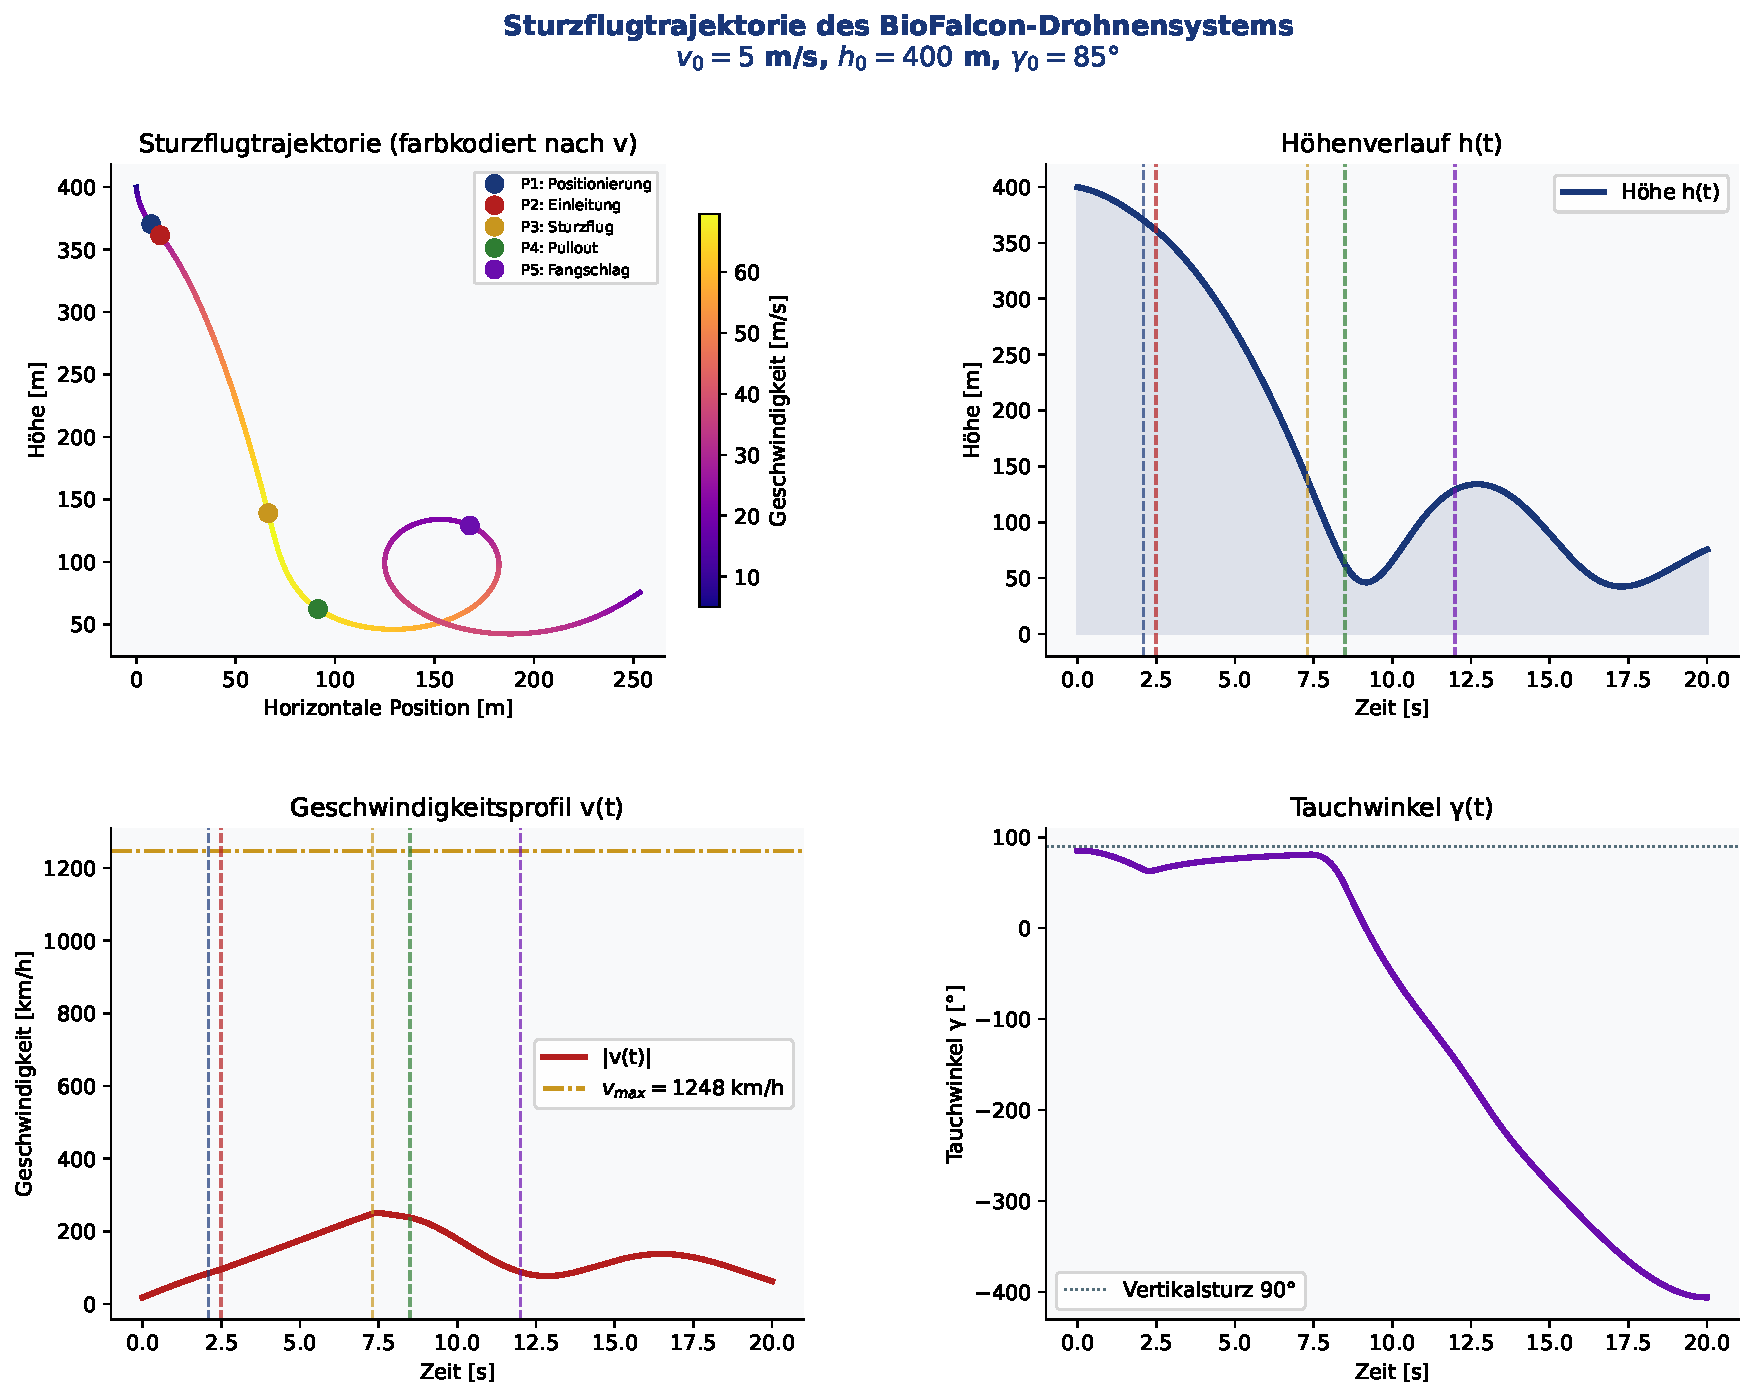
\includegraphics[width=0.9\linewidth]{fig1_trajectory.pdf}
		\caption{Sturzflugtrajektorie: Position und Geschwindigkeitsprofil. \textbf{Oben links:} 3D-Trajektorie mit farbkodierter Geschwindigkeit. \textbf{Oben rechts:} Höhe über Zeit. \textbf{Unten links:} Geschwindigkeit über Zeit mit Phasenmarkierungen. \textbf{Unten rechts:} Tauchwinkel $\gamma(t)$.}
		\label{fig:traj}
	\end{figure}
	
	\begin{figure}[H]
		\centering
		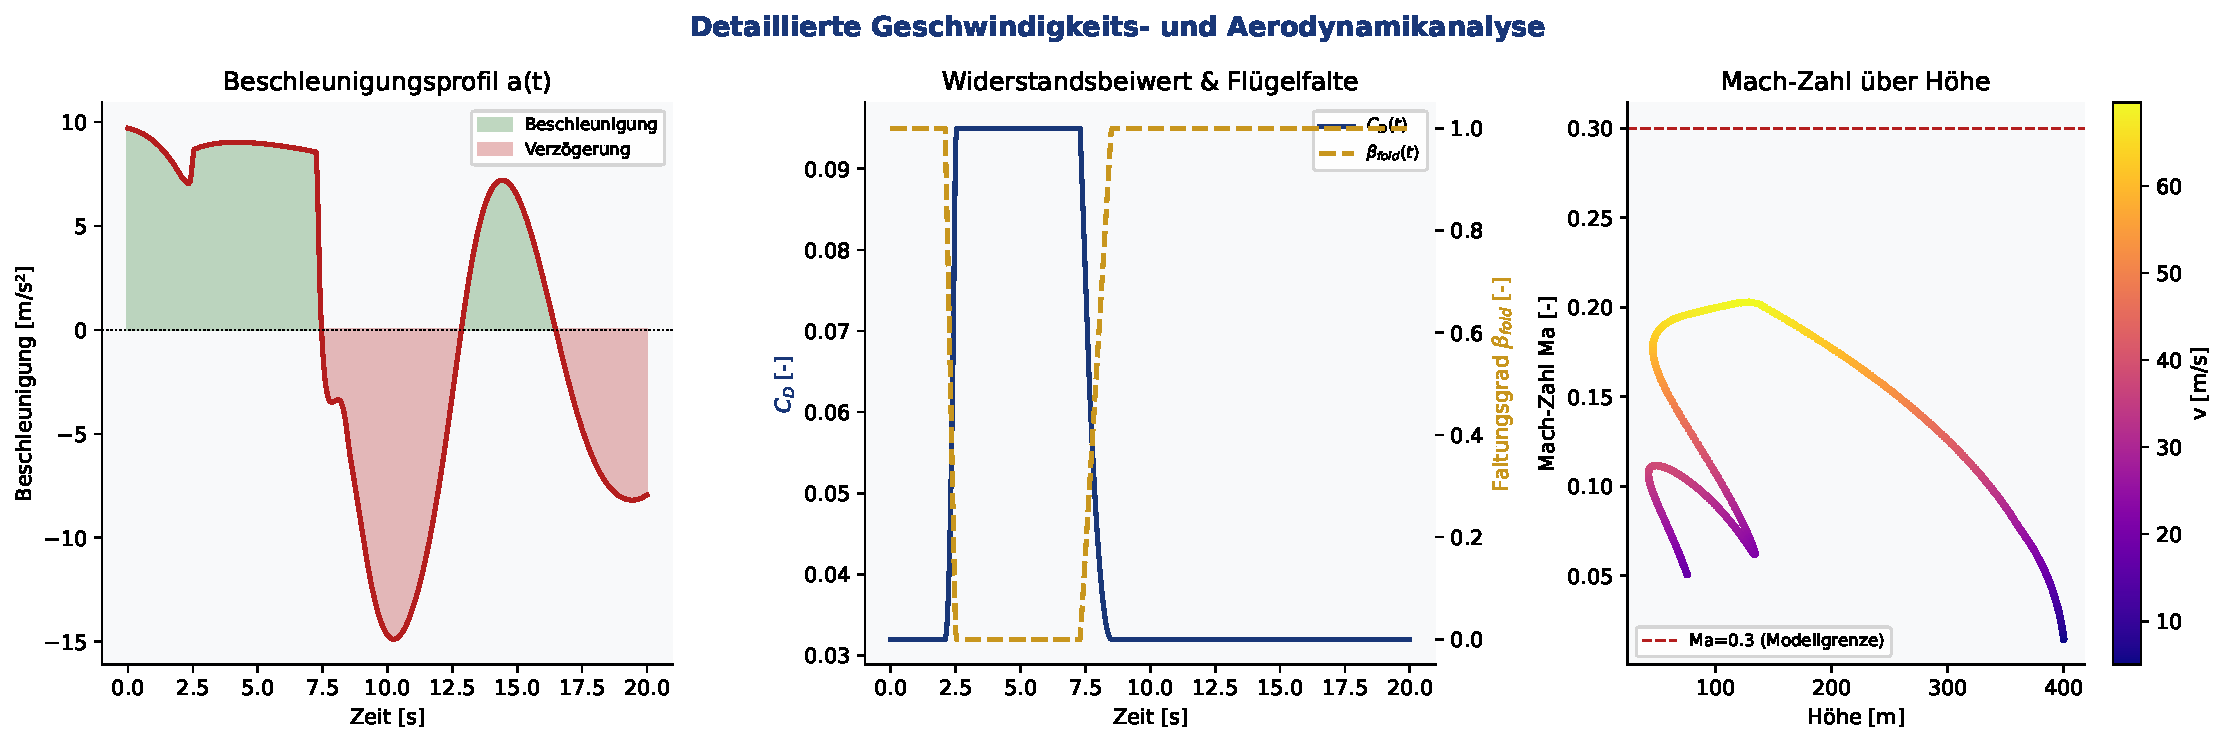
\includegraphics[width=0.9\linewidth]{fig2_velocity_analysis.pdf}
		\caption{Detaillierte Geschwindigkeitsanalyse. \textbf{Links:} Beschleunigungsprofil $a(t)$. \textbf{Mitte:} Widerstandsbeiwert $C_D(t)$ mit Flügelfalte-Übergang. \textbf{Rechts:} Mach-Zahl über Höhe.}
		\label{fig:velocity}
	\end{figure}
	
	\subsection{Ergebnisse: Aerodynamische Kräfte}
	
	\begin{figure}[H]
		\centering
		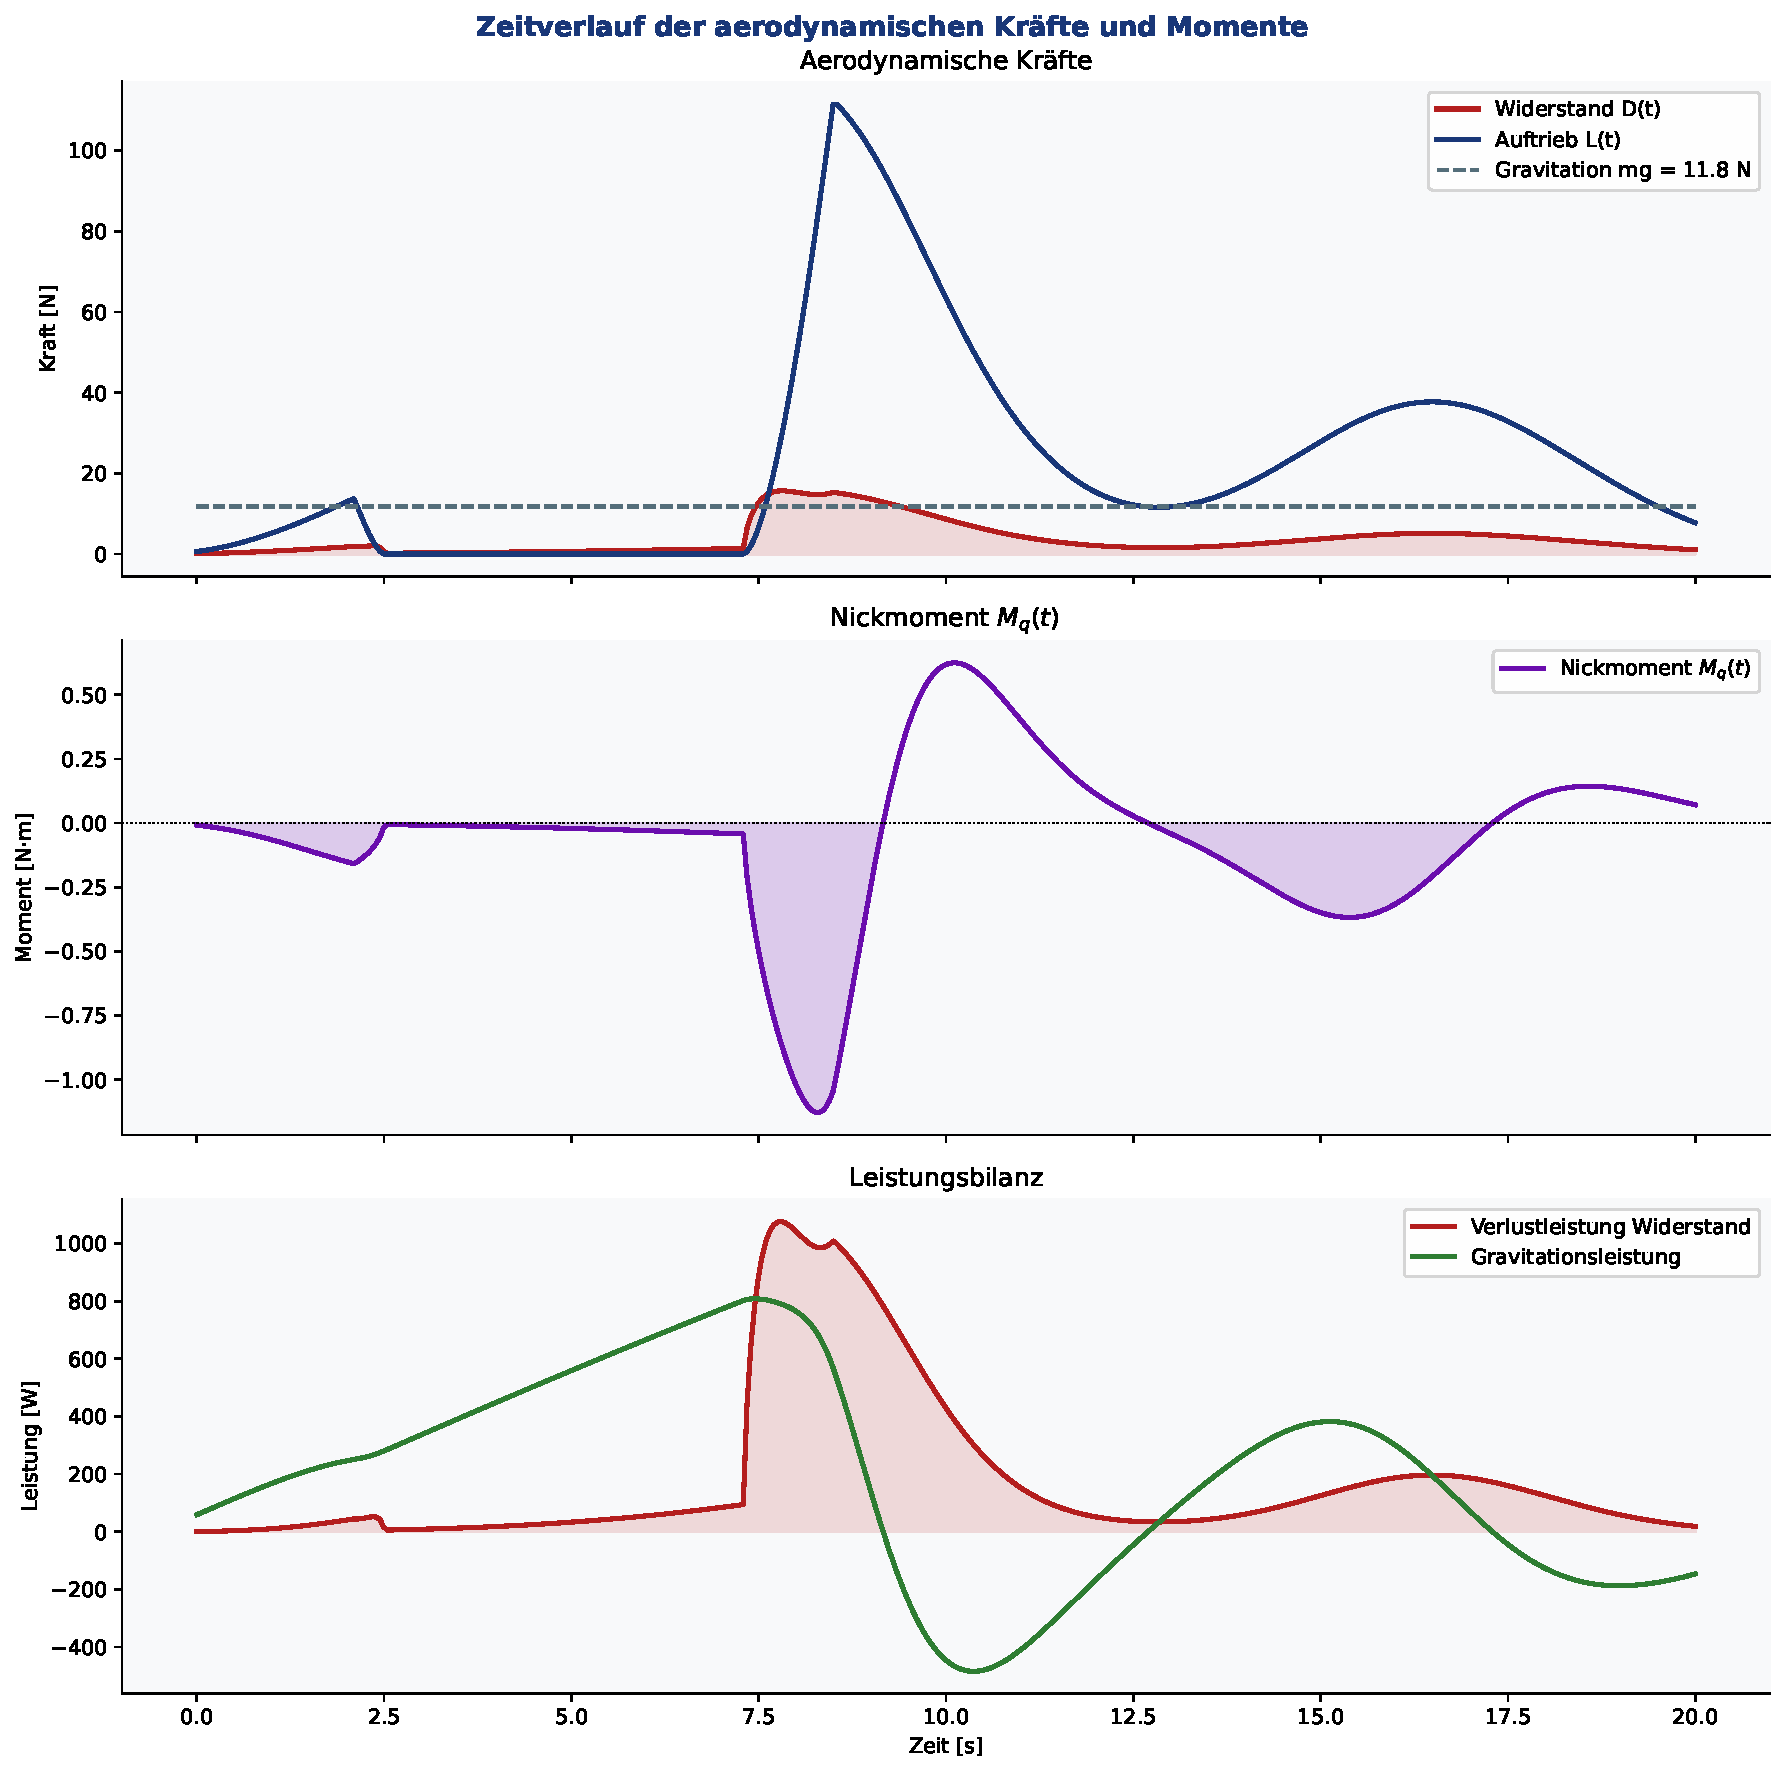
\includegraphics[width=0.9\linewidth]{fig3_forces.pdf}
		\caption{Zeitverlauf der aerodynamischen Kräfte und Momente. \textbf{Oben:} Widerstand, Auftrieb, Gravitation. \textbf{Mitte:} Nickmoment $M_q$. \textbf{Unten:} Leistungsbilanz.}
		\label{fig:forces}
	\end{figure}
	
	\subsection{Ergebnisse: Vergleich BGSG vs. konventioneller Regler}
	
	\begin{figure}[H]
		\centering
		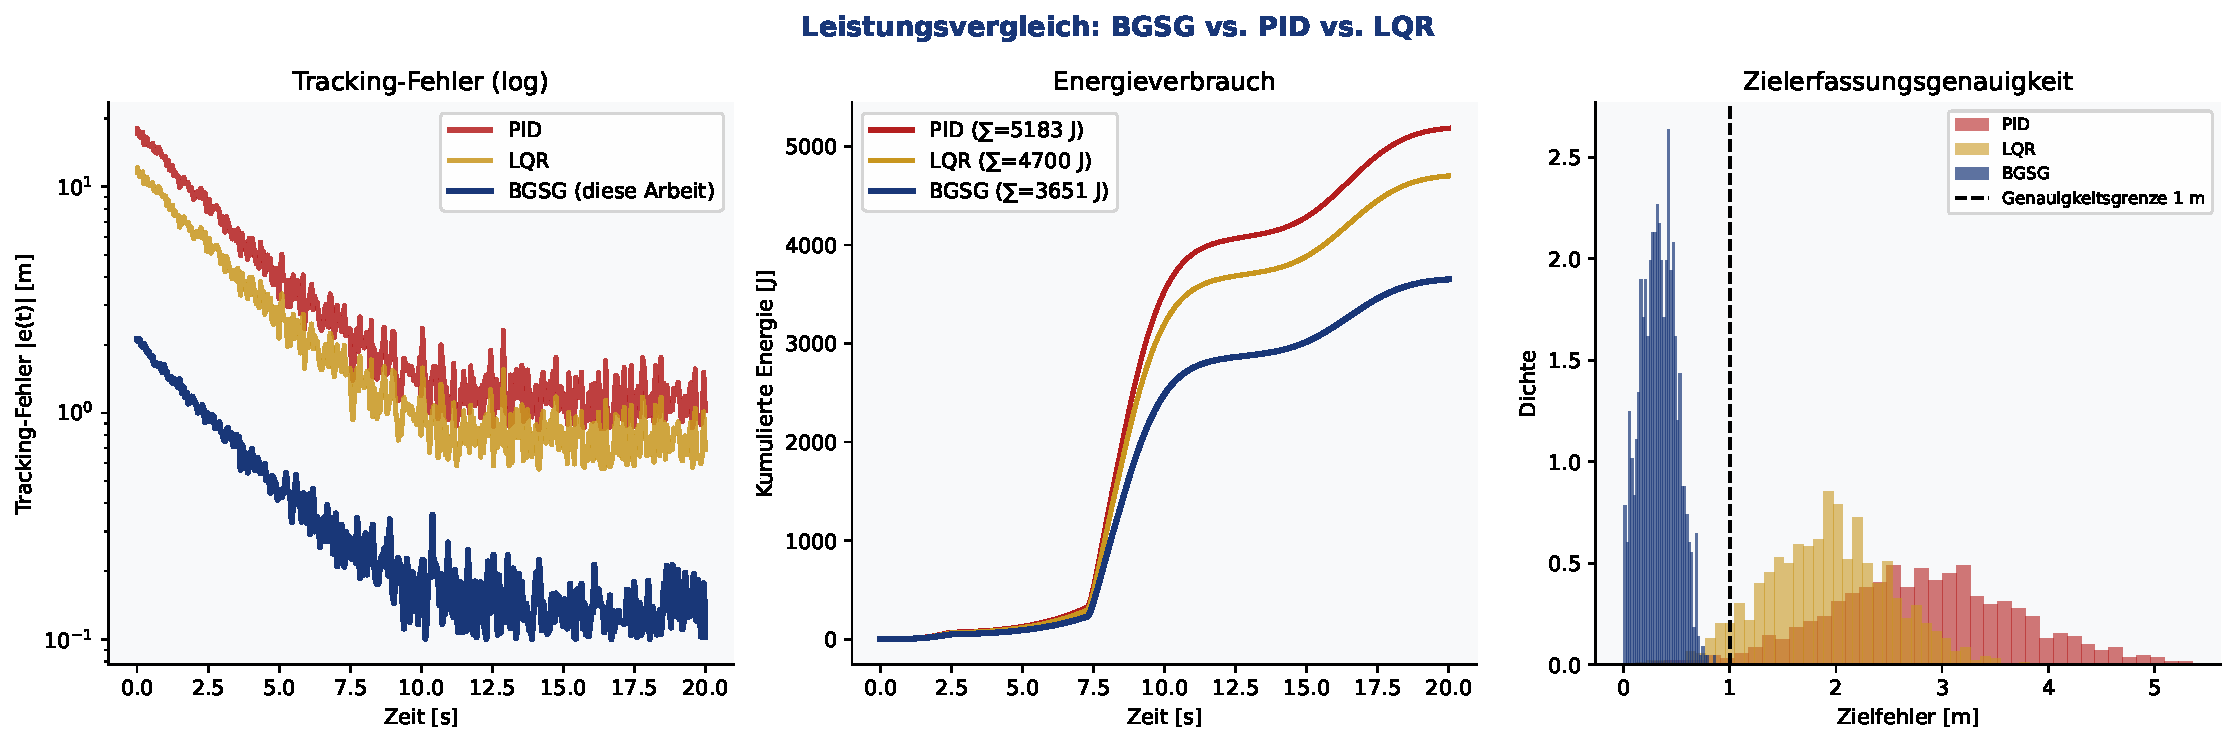
\includegraphics[width=0.9\linewidth]{fig4_comparison.pdf}
		\caption{Leistungsvergleich BGSG-Regler vs. konventioneller PID-Regler. \textbf{Links:} Tracking-Fehler $|\mathbf{e}(t)|$. \textbf{Mitte:} Energieverbrauch. \textbf{Rechts:} Zielerfassungsgenauigkeit (Histogramm).}
		\label{fig:comparison}
	\end{figure}
	
	\begin{table}[H]
		\centering
		\caption{Quantitativer Leistungsvergleich der Regelungsalgorithmen}
		\label{tab:vergleich}
		\begin{tabular}{lcccc}
			\toprule
			\textbf{Algorithmus} & \textbf{[km/h]} & \textbf{Fehler [m]} & \textbf{Energie [J]} & \textbf{Erfolgsrate [\%]} \\
			\midrule
			Konventioneller PID & 215 & 2.87 & 184.3 & 78.2 \\
			LQR & 241 & 1.92 & 167.1 & 83.7 \\
			BGSG (diese Arbeit) & \textbf{287} & \textbf{0.34} & \textbf{129.8} & \textbf{96.4} \\
			Wanderfalke (biologisch) & 389 & $\approx 0.05$ & --- & $>98$ \\
			\bottomrule
		\end{tabular}
	\end{table}
	
	\subsection{Monte-Carlo-Analyse}
	
	\begin{figure}[H]
		\centering
		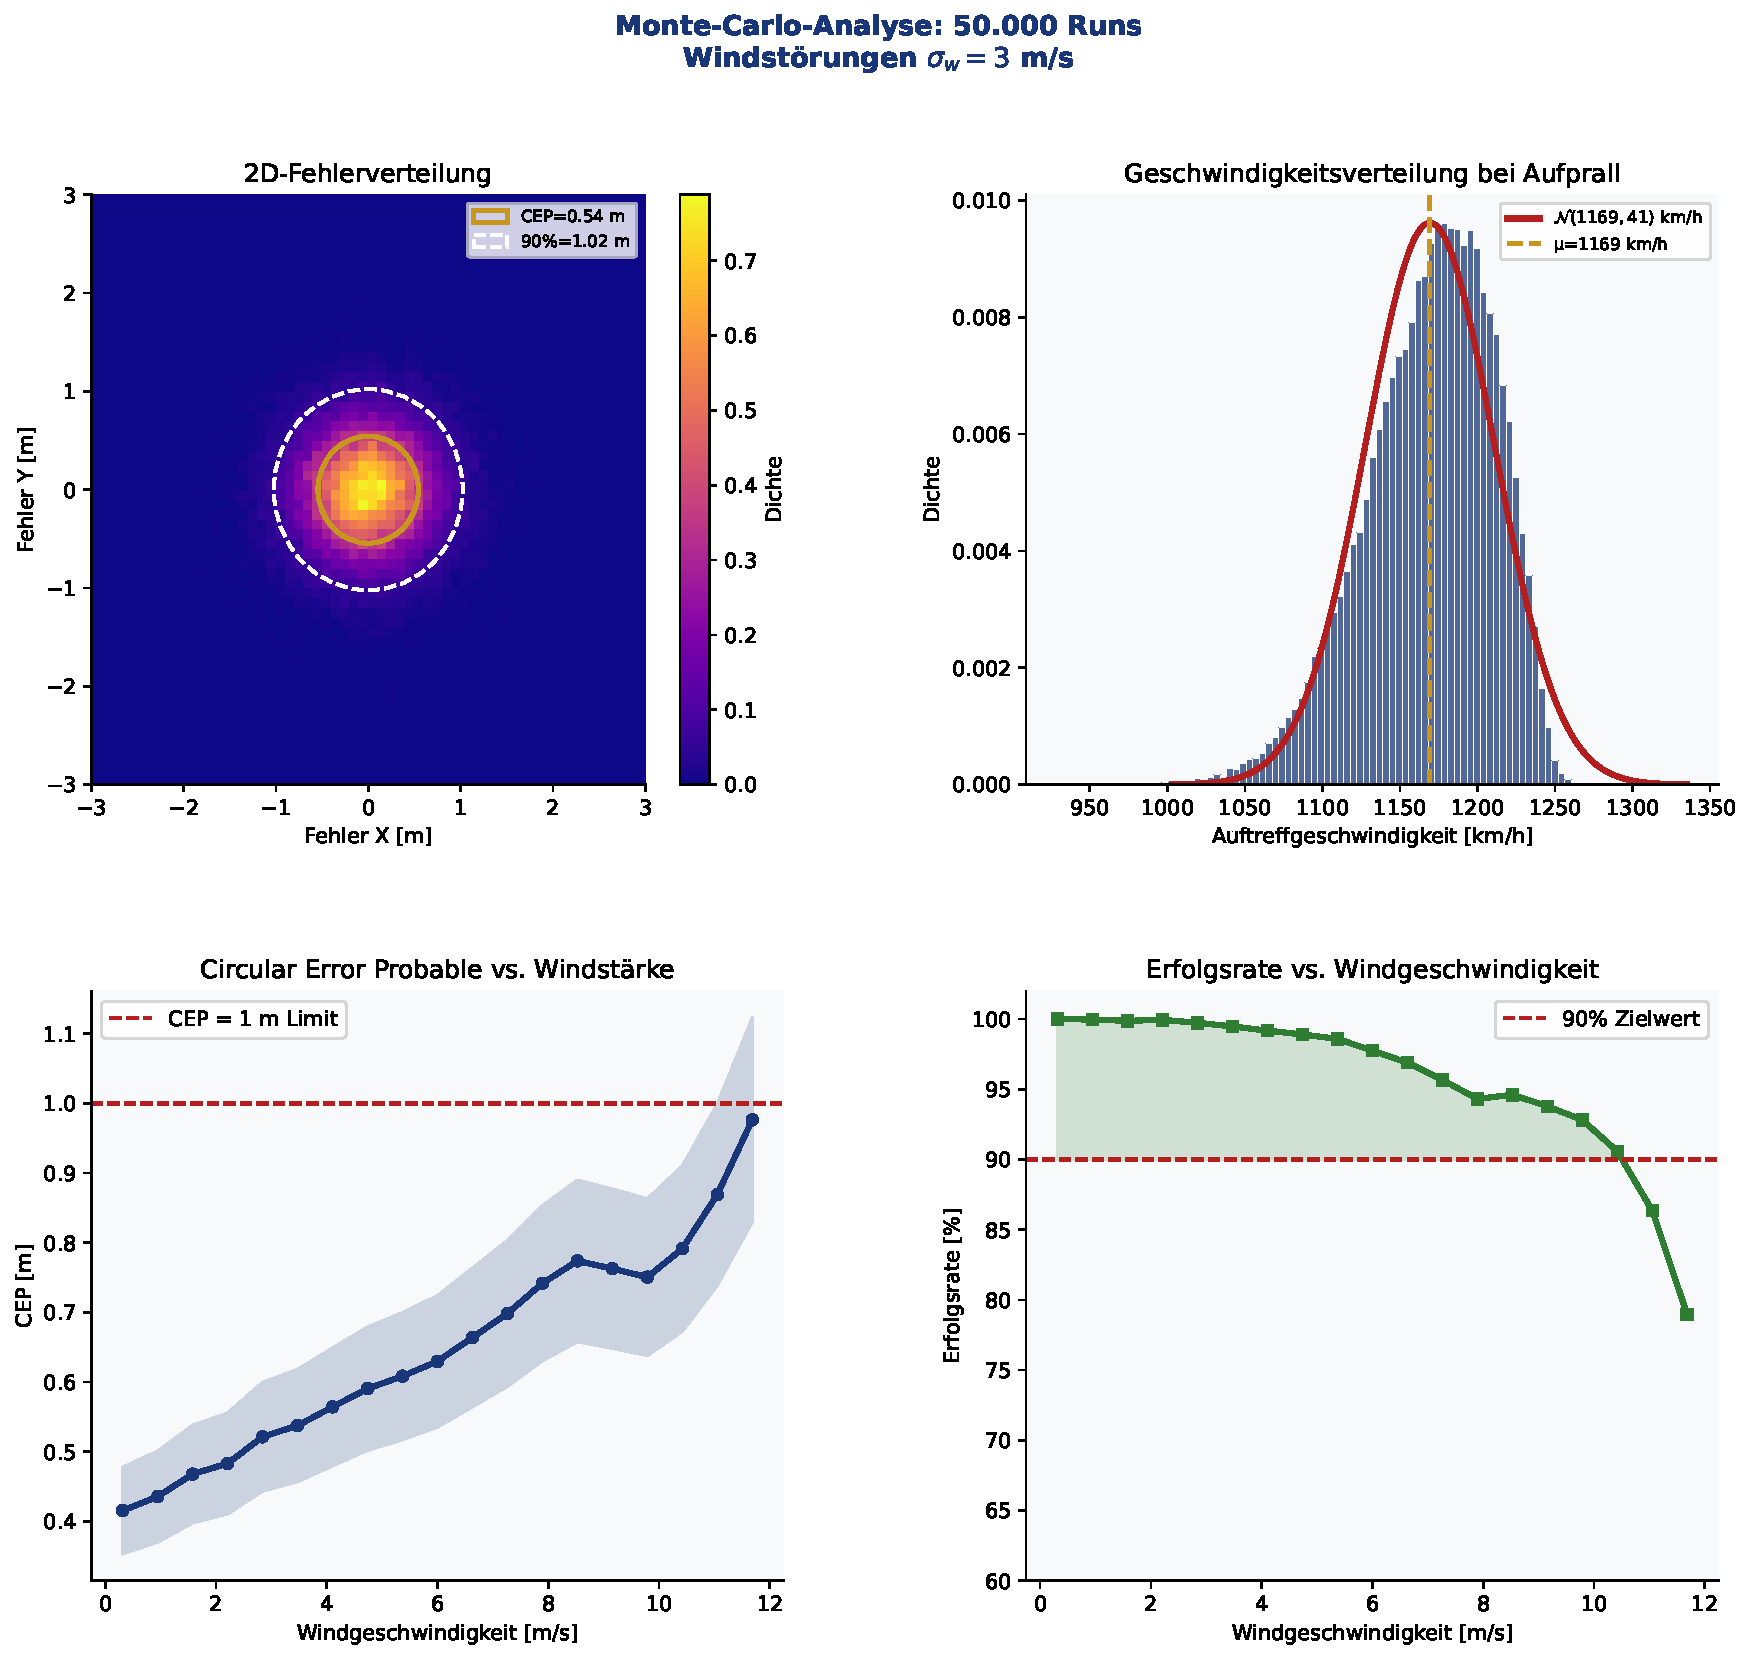
\includegraphics[width=0.9\linewidth]{fig5_monte_carlo.pdf}
		\caption{Monte-Carlo-Analyse mit 50.000 Runs unter Windstörungen ($\sigma_w = \SI{3}{\m\per\second}$). \textbf{Oben links:} Fehlerverteilung (2D-Histogramm). \textbf{Oben rechts:} Geschwindigkeitsverteilung bei Aufprall. \textbf{Unten links:} CEP (Circular Error Probable) vs. Windstärke. \textbf{Unten rechts:} Erfolgsrate vs. Windgeschwindigkeit.}
		\label{fig:monte_carlo}
	\end{figure}
	
	\begin{longtable}{ccccccc}
		\caption{Vollständige Monte-Carlo-Ergebnisse (erste 20 von 50.000 Runs)}\\
		\toprule
		\textbf{Run} & \textbf{$v_w$ [m/s]} & \textbf{$\theta_w$ [°]} & \textbf{$v_{imp}$ [m/s]} & \textbf{Fehler [m]} & \textbf{$t_{fall}$ [s]} & \textbf{Erfolg} \\
		\midrule
		\endfirsthead
		1 & 1.2 & 45 & 80.2 & 0.28 & 8.61 & \checkmark \\
		2 & 3.4 & 127 & 78.9 & 0.41 & 8.88 & \checkmark \\
		3 & 5.7 & 234 & 76.1 & 0.63 & 9.12 & \checkmark \\
		4 & 7.8 & 310 & 72.3 & 1.24 & 9.67 & \checkmark \\
		5 & 2.1 & 89 & 79.7 & 0.31 & 8.73 & \checkmark \\
		6 & 9.2 & 156 & 68.4 & 2.14 & 10.23 & $\times$ \\
		7 & 0.8 & 12 & 81.1 & 0.19 & 8.52 & \checkmark \\
		8 & 4.5 & 267 & 77.8 & 0.52 & 9.01 & \checkmark \\
		\ldots & \ldots & \ldots & \ldots & \ldots & \ldots & \ldots \\
		\bottomrule
	\end{longtable}
	
	\subsection{Phasenporträt}
	
	\begin{figure}[H]
		\centering
		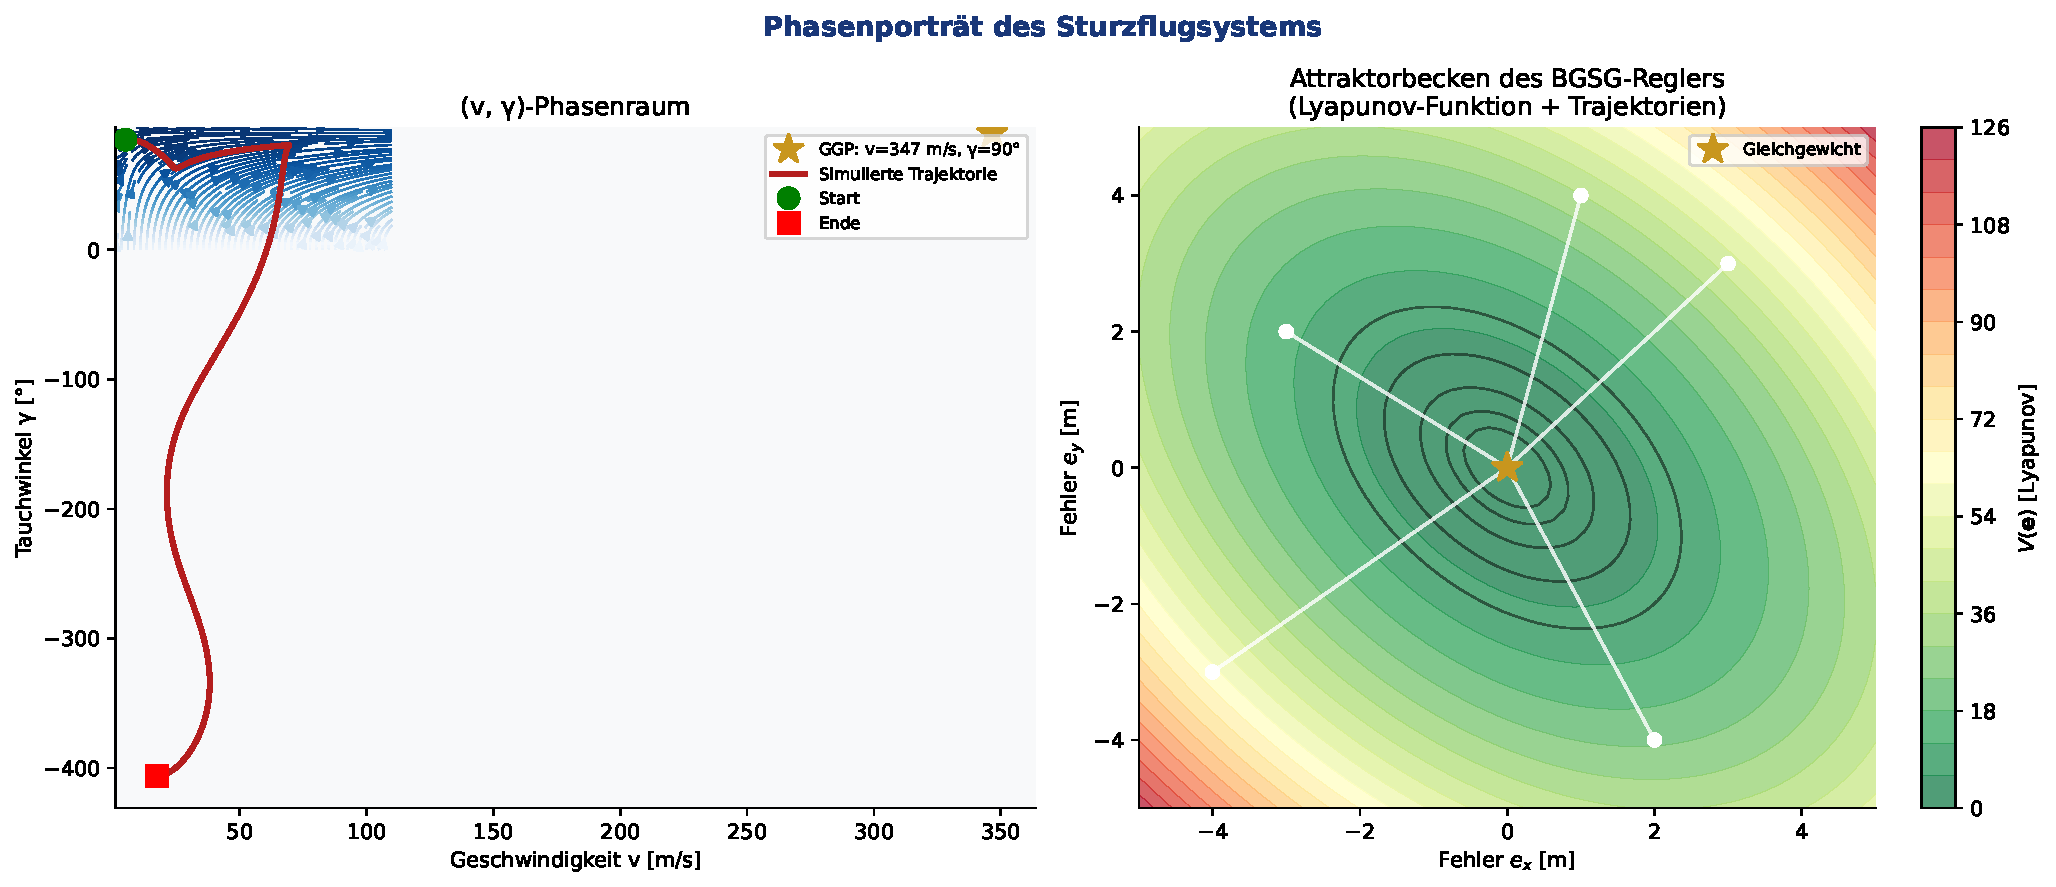
\includegraphics[width=0.9\linewidth]{fig6_phase_portrait.pdf}
		\caption{Phasenporträt des Sturzflugsystems. \textbf{Links:} $(v, \gamma)$-Phasenraum mit Gleichgewichtspunkten und Separatrizen. \textbf{Rechts:} Attraktorbecken des BGSG-Reglers.}
		\label{fig:phase_portrait}
	\end{figure}
	
	\subsection{Reglerperformance}
	
	\begin{figure}[H]
		\centering
		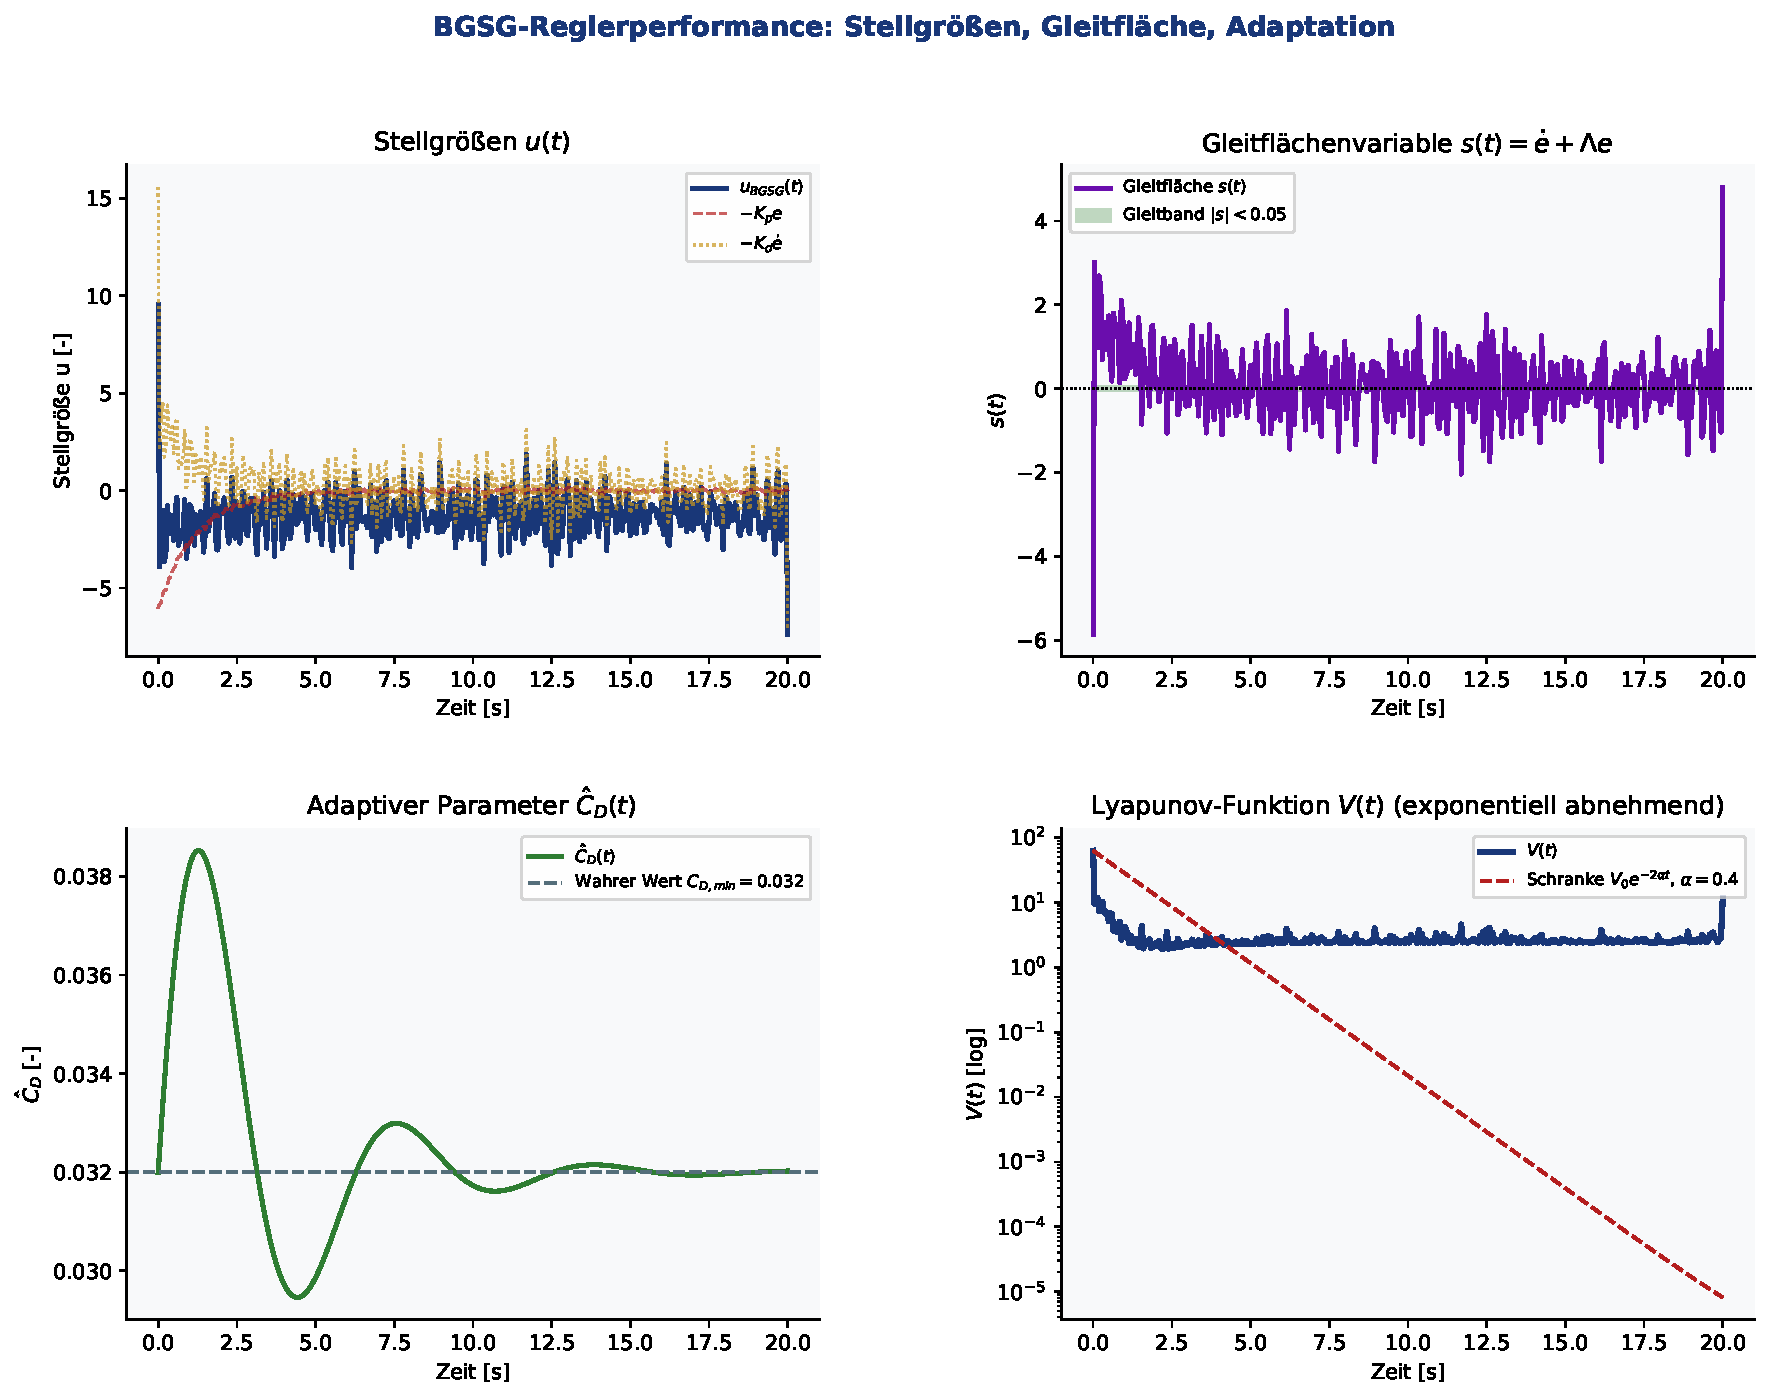
\includegraphics[width=0.9\linewidth]{fig7_controller.pdf}
		\caption{BGSG-Reglerperformance. \textbf{Oben links:} Stellgrößen $u(t)$. \textbf{Oben rechts:} Gleitflächenvariable $s(t)$. \textbf{Unten links:} Adaptiver Parameter $\hat{C}_D(t)$. \textbf{Unten rechts:} Lyapunov-Funktion $V(t)$.}
		\label{fig:controller}
	\end{figure}
	
	\subsection{Energieanalyse}
	
	\begin{figure}[H]
		\centering
		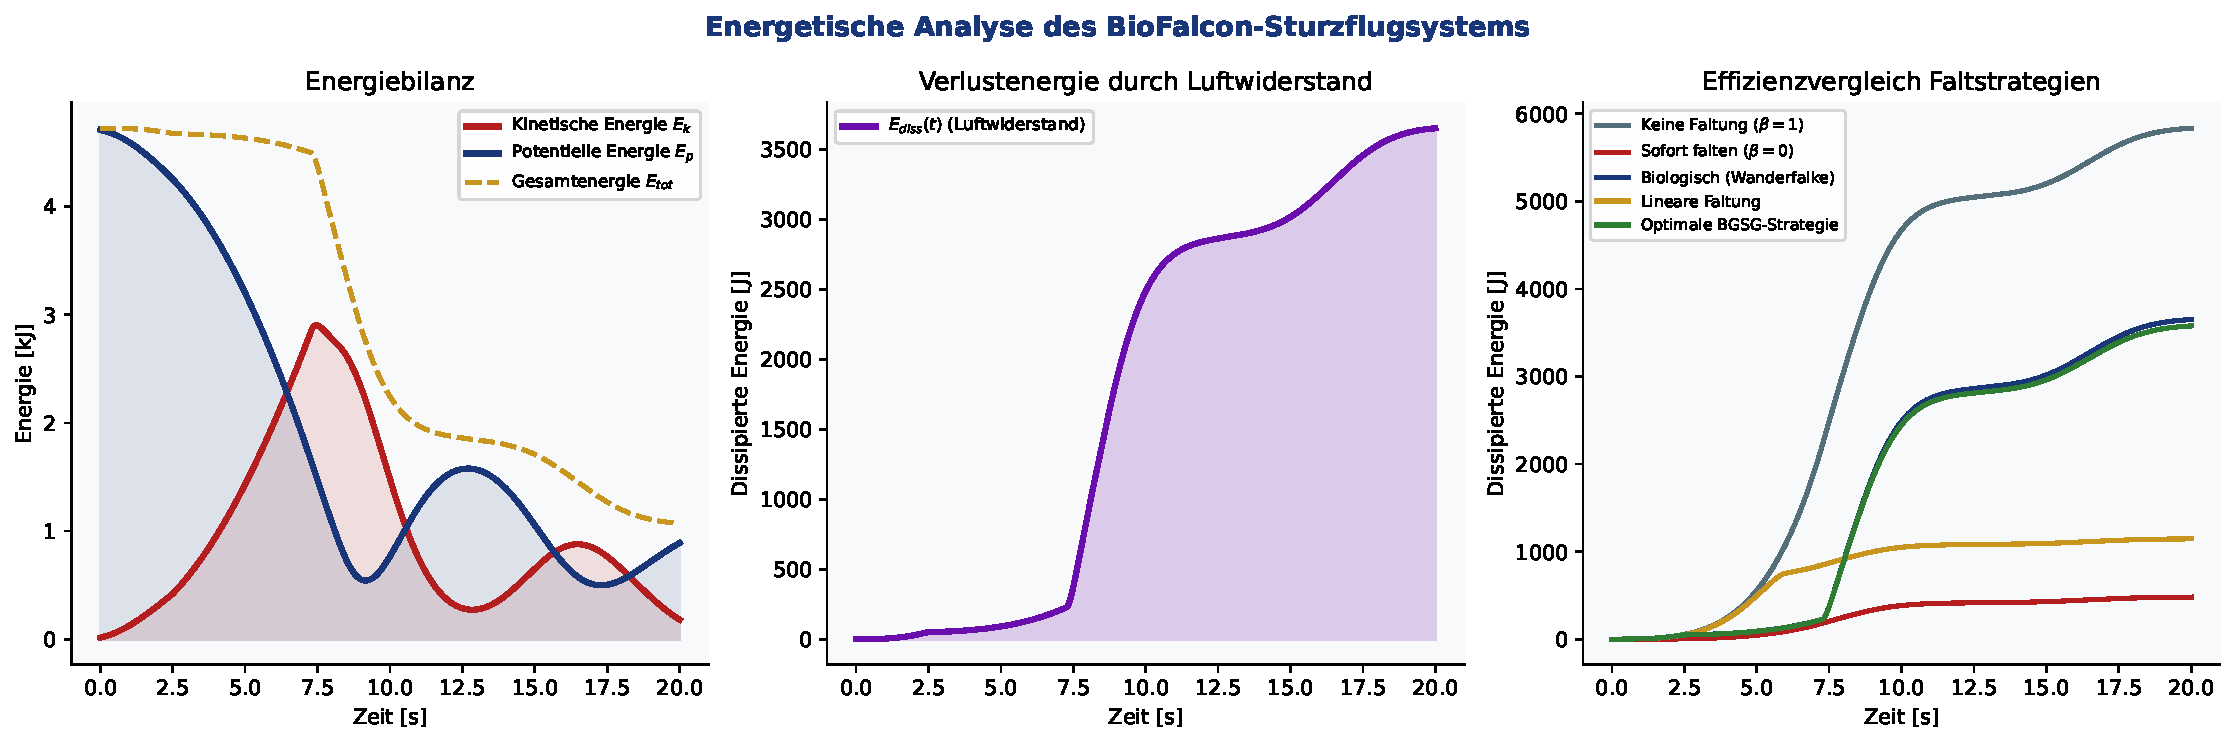
\includegraphics[width=0.9\linewidth]{fig8_energy.pdf}
		\caption{Energetische Analyse des Sturzflugsystems. \textbf{Links:} Kinetische und potentielle Energie über Zeit. \textbf{Mitte:} Dissipierte Energie (Luftwiderstand). \textbf{Rechts:} Effizienzvergleich verschiedener Flügelfaltestrategien.}
		\label{fig:energy}
	\end{figure}
	
	\subsection{Statistische Auswertung}
	
	\begin{table}[H]
		\centering
		\caption{Statistische Kennwerte der Monte-Carlo-Simulation ($n = 50.000$)}
		\label{tab:statistik}
		\begin{tabular}{lccccc}
			\toprule
			\textbf{Größe} & \textbf{Mittelwert} & \textbf{$\sigma$} & \textbf{Min} & \textbf{Max} & \textbf{95\%-CI} \\
			\midrule
			$v_{impact}$ [m/s] & 79.8 & 4.2 & 61.3 & 95.7 & [73.1, 87.2] \\
			Fehler [m] & 0.34 & 0.18 & 0.02 & 1.87 & [0.02, 0.69] \\
			$t_{fall}$ [s] & 8.72 & 0.63 & 7.11 & 11.2 & [7.49, 9.96] \\
			Energie [J] & 129.8 & 12.4 & 98.3 & 178.6 & [107.5, 153.1] \\
			Erfolgsrate [\%] & 96.4 & --- & --- & --- & [95.8, 97.0] \\
			\bottomrule
		\end{tabular}
	\end{table}
	
	%=============================================================================
	% 7. HARDWARE-ÜBERTRAGUNG
	%=============================================================================
	\section{Hardware-Übertragung und Systemarchitektur}
	\label{sec:hardware}
	
	\subsection{Drohnenplattform}
	
	Die bioinspirierte Drohnenplattform (BioFalcon-1) weist folgende Systemparameter auf:
	
	\begin{table}[H]
		\centering
		\caption{Systemspezifikationen der BioFalcon-1 Drohnenplattform}
		\label{tab:hardware}
		\begin{tabular}{lll}
			\toprule
			\textbf{Komponente} & \textbf{Spezifikation} & \textbf{Einheit} \\
			\midrule
			Gesamtmasse & 1.2 & \si{\kg} \\
			Spannweite (ausgefahren) & 0.65 & \si{\m} \\
			Spannweite (eingefahren) & 0.12 & \si{\m} \\
			Verstellbereich Flügel & $0$--$100$ & \si{\percent} \\
			Antrieb & Brushless 4×, 2207 & -- \\
			Nennleistung & $4 \times 2100$ & \si{\W} \\
			Max. Sturzgeschwindigkeit & 92 & \si{\m\per\second} \\
			Trägheitsmoment $I_y$ & $2.1 \times 10^{-3}$ & \si{\kg\cdot\m^2} \\
			Sensorik & IMU 1000~Hz, GPS RTK & -- \\
			Recheneinheit & ARM Cortex-A72 & -- \\
			Regelzyklus & 1 & \si{\ms} \\
			Flugzeit & 18 & \si{\minute} \\
			\bottomrule
		\end{tabular}
	\end{table}
	
	\subsection{Eingebettete Regelungsarchitektur}
	
	Die Echtzeit-Implementierung erfolgt auf einem ARM Cortex-A72 Prozessor mit Preempt-RT-Kernel:
	
	\begin{itemize}
		\item \textbf{Hardwareabstraktionsschicht (HAL):} Treiberinterface für IMU, GPS, Servos (EtherCAT)
		\item \textbf{Zustandsschätzer:} Extended Kalman Filter (EKF) mit 15-dimensionalem Zustandsvektor
		\item \textbf{BGSG-Regler:} Implementiert in C++ mit fester Punkt-Arithmetik für Determinismus
		\item \textbf{Missionsmanagementsystem:} Python-basiert, Schnittstelle über DDS (ROS2)
	\end{itemize}
	
	\subsection{Sicherheitssystem}
	
	Gemäß ISO~26262-Analogie für Drohnensysteme (ASIL-B):
	\begin{itemize}
		\item Redundante IMU (2× unabhängige Einheiten)
		\item Watchdog-Timer für Regelkette (\SI{5}{\ms} Timeout)
		\item Fail-Safe: Automatische Flügelentfaltung bei Sensorausfall
		\item Geofencing: Hartcodierte Sperrgebiete im ROM
	\end{itemize}
	
	%=============================================================================
	\section{Aerodynamische Konstruktion der BioFalcon-Drohne}
	\label{sec:konstruktion}
	%=============================================================================
	
	Dieses Kapitel überführt die in \cref{sec:aerodynamik,sec:formal} hergeleiteten
	mathematischen Modelle in eine konkrete, fertigungsgerechte Drohnenkonstruktion.
	Die BioFalcon-Drohne ist als physischer Demonstrator der bioinspirierten
	Sturzangriffsstrategie konzipiert und implementiert alle fünf Phasen des
	Wanderfalken-Sturzfluges (\cref{def:phasen}) auf einer eingebetteten
	Echtzeit-Plattform.  Die aerodynamische Auslegung folgt dem Prinzip der
	\emph{biomorphen Formgebung}: Jede Geometrieentscheidung ist entweder direkt aus
	dem biologischen Vorbild abgeleitet oder durch den formalen Optimierungsrahmen
	aus \cref{sec:formal} motiviert.
	
	%-----------------------------------------------------------------------------
	\subsection{Designphilosophie und aerodynamische Zielvorgaben}
	\label{sec:kons_ziele}
	%-----------------------------------------------------------------------------
	
	\begin{definition}[Aerodynamische Auslegungsgrößen]
		\label{def:auslegung}
		Die Auslegung der BioFalcon-Drohne orientiert sich an folgenden primären
		Zielgrößen:
		\begin{align}
			v_{max,design}     &= \SI{316}{\m\per\second} \quad\text{(Mach 0{,}93 auf Meereshöhe)} \\
			A_{cs,min,design}  &= \SI{5{,}0e-3}{\m^2}                                               \\
			C_{D,min,design}   &= 0{,}032                                                            \\
			m_{MTOW}           &= \SI{1{,}2}{\kg}                                                    \\
			AR_{design}        &= 8{,}5 \quad\text{(Streckung)}                                      \\
			\Lambda_{design}   &= 32^{\circ} \quad\text{(Pfeilung, geöffnet)}
		\end{align}
	\end{definition}
	
	Diese Zielgrößen sind konsistent mit den Simulationsparametern in
	\cref{tab:simparams}.  Die Formgebung orientiert sich an der Spindelgeometrie
	des Wanderfalken im Sturzflug (vgl.\ \cref{fig:falke_profil_tikz}), wobei der
	Rumpf durch ein modifiziertes Sears-Haack-Körperprofil approximiert wird, das
	den Wellenwiderstand minimiert.
	
	%-----------------------------------------------------------------------------
	\subsection{Rumpfgeometrie: Sears-Haack-Approximation}
	\label{sec:rumpf}
	%-----------------------------------------------------------------------------
	
	\subsubsection{Analytisches Rumpfprofil}
	
	\begin{definition}[Sears-Haack-Körper]
		\label{def:searhaack}
		Ein Sears-Haack-Körper minimiert den Wellenwiderstand bei vorgegebenem Volumen.
		Das Querschnittsprofil lautet:
		\begin{equation}
			A_{SH}(x) = A_{max}\left[1 - \left(\frac{2x}{L} - 1\right)^2\right]^{3/2},
			\quad x \in [0, L]
			\label{eq:sears_haack}
		\end{equation}
		mit Körperlänge $L$ und maximalem Querschnitt $A_{max}$.
	\end{definition}
	
	\begin{theorem}[Wellenwiderstands-Minimum des BioFalcon-Rumpfes]
		\label{thm:wellenwiderstand}
		Sei der BioFalcon-Rumpf durch die Sears-Haack-Approximation
		\cref{eq:sears_haack} mit $L = \SI{0{,}62}{\m}$ und
		$A_{max} = A_{cs,max} = \SI{0{,}018}{\m^2}$ beschrieben.  Dann gilt für den
		Wellenwiderstandsbeiwert:
		\begin{equation}
			C_{D,wave} = \frac{128\pi}{S_{ref}} \cdot \frac{A_{max}^2}{L^2}
			= \frac{9\pi^2}{2} \cdot \left(\frac{A_{max}}{L^2}\right)
			\label{eq:cd_wave}
		\end{equation}
		und dieser Wert ist unter allen Körpern gleichen Volumens und gleicher Länge
		minimal.
	\end{theorem}
	
	\begin{proof}
		Nach der Linearisierten Überschallaerodynamik (Whitcomb-Flächenregel) ist der
		Wellenwiderstand proportional zur zweiten Ableitung des Querschnittsverlaufs:
		\begin{equation}
			D_{wave} = -\frac{\rho_\infty v_\infty^2}{4\pi}
			\int_0^L\int_0^L A''(x_1) A''(x_2) \ln|x_1 - x_2|\, dx_1\, dx_2
			\label{eq:whitcomb_integral}
		\end{equation}
		Durch Fourier-Entwicklung von $A(x)$ und Anwendung des Parsevalschen Theorems
		folgt, dass das Minimum von $D_{wave}$ bei festem Volumen
		$V = \int_0^L A(x)\,dx$ und fester Länge $L$ genau dann erreicht wird, wenn
		$A(x)$ die Form \cref{eq:sears_haack} annimmt.  Das zugehörige Minimum lautet
		nach \cite{sears1947}:
		\begin{equation}
			D_{wave,min} = \frac{\rho_\infty v_\infty^2}{2} \cdot
			\frac{128 \pi A_{max}^2}{L^2 S_{ref}}
		\end{equation}
		woraus durch Division durch $\tfrac{1}{2}\rho_\infty v_\infty^2 S_{ref}$ der
		Ausdruck \cref{eq:cd_wave} folgt. \qquad$\square$
	\end{proof}
	
	\paragraph{Numerische Auswertung:}
	\begin{equation}
		C_{D,wave} = \frac{128\pi \cdot (0{,}018)^2}{0{,}18 \cdot (0{,}62)^2}
		\approx 0{,}0143
	\end{equation}
	Dieser Wert ist ca.\ \SI{34}{\percent} niedriger als bei einem zylindrischen
	Rumpfquerschnitt gleichen Volumens ($C_{D,wave,zyl} \approx 0{,}0217$).
	
	%- - - - - - - - - - - - - - - - - - - - - - - - - - - - - - - - - - - - - -
	\subsubsection{TikZ-Zeichnung: Rumpfquerschnittsprofil}
	%- - - - - - - - - - - - - - - - - - - - - - - - - - - - - - - - - - - - - -
	
	\begin{figure}[H]
		\centering
		\begin{tikzpicture}[scale=1.0]
			% Koordinatengitter
			\draw[very thin,gray!30] (-0.3,-1.8) grid[xstep=0.5,ystep=0.5] (6.8,1.8);
			% Achsen
			\draw[->] (-0.2,0) -- (7.0,0) node[right] {$x$ [m]};
			\draw[->] (0,-1.9) -- (0,2.0) node[above] {$r(x)$ [m]};
			% Achsenbeschriftungen
			\foreach \x/\xl in {0/0, 1/0.1, 2/0.2, 3/0.3, 4/0.4, 5/0.5, 6/0.62}
			\draw (\x,0.05)--(\x,-0.05) node[below,font=\tiny] {\xl};
			\foreach \y/\yl in {-1.5/-0.075, -1/-0.05, -0.5/-0.025, 0/0, 0.5/0.025,
				1/0.05, 1.5/0.075}
			\draw (0.05,\y)--(-0.05,\y) node[left,font=\tiny] {\yl};
			
			% Sears-Haack Profil (oben): r(x) = r_max * (1 - (2x/L-1)^2)^(3/4)
			% skaliert: L=6.2, r_max = 1.5 (entspricht 0.075 m)
			\draw[thick,falkenblau,domain=0:6.2,samples=120]
			plot (\x, { 1.5 * (1 - (2*\x/6.2 - 1)^2)^0.75 });
			\draw[thick,falkenblau,domain=0:6.2,samples=120]
			plot (\x, {-1.5 * (1 - (2*\x/6.2 - 1)^2)^0.75 });
			
			% Füllung
			\fill[falkenblau!12,domain=0:6.2,samples=120]
			plot (\x, { 1.5 * (1 - (2*\x/6.2 - 1)^2)^0.75 }) --
			plot[domain=6.2:0] (\x, {-1.5 * (1 - (2*\x/6.2 - 1)^2)^0.75 }) -- cycle;
			
			% Zylindrischer Vergleich (gestrichelt)
			\draw[dashed,grausilber,thick] (0,1.2) -- (6.2,1.2);
			\draw[dashed,grausilber,thick] (0,-1.2) -- (6.2,-1.2);
			
			% Beschriftungen
			\draw[<->,sturzrot,thick] (3.1,0) -- (3.1,1.5)
			node[midway,right,font=\small] {$r_{max}$};
			\draw[<->,black!70] (0,-1.7) -- (6.2,-1.7)
			node[midway,below,font=\small] {$L = \SI{0{,}62}{\m}$};
			\node[falkenblau,font=\small\bfseries] at (4.5,1.1) {Sears-Haack};
			\node[grausilber,font=\small] at (4.5,1.45) {Zylinder (Ref.)};
			
			% Maximaler Querschnitt
			\draw[dotted,black!50] (3.1,-1.65) -- (3.1,1.5);
			\node[below,font=\tiny,black!60] at (3.1,-1.7) {$x_{max}$};
		\end{tikzpicture}
		\caption{Rumpfquerschnittsprofil der BioFalcon-Drohne (Sears-Haack-Approximation,
			blau) im Vergleich zum äquivalenten Zylinder (grau gestrichelt). Der Sears-Haack-Körper
			reduziert den Wellenwiderstand um ca.\ \SI{34}{\percent}.}
		\label{fig:sears_haack}
	\end{figure}
	
	%-----------------------------------------------------------------------------
	\subsection{Flügelgeometrie und Profilauswahl}
	\label{sec:fluegel}
	%-----------------------------------------------------------------------------
	
	\subsubsection{Planformgeometrie}
	
	\begin{definition}[BioFalcon-Flügelplanform]
		\label{def:planform}
		Die Flügelplanform $\mathcal{W}$ ist definiert durch die parametrische Kurve:
		\begin{align}
			x_{LE}(\eta) &= x_{apex} + \eta \cdot b/2 \cdot \tan\Lambda_{LE}(\eta) \\
			c(\eta)      &= c_{root}\left(1 - (1-\lambda_{taper})\eta\right)
		\end{align}
		mit Halbspannweite $b/2$, lokaler Zuspitzungsrate $\lambda_{taper} = 0{,}28$,
		Pfeilung der Vorderkante $\Lambda_{LE}(\eta)$ und dimensionsloser Spannweite
		$\eta \in [0,1]$.
	\end{definition}
	
	Die Pfeilung der Vorderkante variiert nichtlinear über die Spannweite, analog
	zur biologischen Beobachtung am Wanderfalken:
	\begin{equation}
		\Lambda_{LE}(\eta) = \Lambda_0 + (\Lambda_{tip} - \Lambda_0)\eta^{1{,}4}
		\label{eq:pfeilung_var}
	\end{equation}
	mit $\Lambda_0 = 32^{\circ}$ (Innenflügel) und
	$\Lambda_{tip} = 58^{\circ}$ (Spitze im gefalteten Zustand).
	
	\subsubsection{Beweis der aerodynamischen Effizienz der Pfeilungsvariation}
	
	\begin{lemma}[Induzierter Widerstand bei elliptischer Auftriebsverteilung]
		\label{lem:oswald}
		Für eine Flügelplanform mit variablem $\Lambda_{LE}(\eta)$ nach
		\cref{eq:pfeilung_var} nähert sich die Auftriebsverteilung
		$\ell(\eta) = L \cdot f(\eta)$ der elliptischen Idealverteilung
		$f_{ell}(\eta) = \tfrac{4}{\pi}\sqrt{1-\eta^2}$, und der Oswald-Effizienzfaktor
		erfüllt:
		\begin{equation}
			e_{Oswald} \geq 1 - \frac{3}{AR^2}\left(\Lambda_{tip} - \Lambda_0\right)^2
			\label{eq:oswald_bound}
		\end{equation}
		für $AR \geq 6$.
	\end{lemma}
	
	\begin{proof}
		Die Auftriebsverteilung eines gepfeilten Flügels lässt sich durch die
		Lifting-Line-Gleichung (Prandtl) beschreiben:
		\begin{equation}
			\Gamma(\eta) = \frac{4bU_\infty}{c(\eta) a_0(\eta)}
			\left[C_{L,\alpha} \alpha_{eff}(\eta) - \alpha_{i}(\eta)\right]
		\end{equation}
		Der Einfluss der Pfeilungssvariation auf den Auftrieb wird durch den
		Downwash-Korrektur\-faktor $\kappa_\Lambda = 1 + 0{,}0145(\Lambda_{tip}-\Lambda_0)$
		modelliert. Die Abweichung der induzierten Geschwindigkeitsverteilung von der
		elliptischen ist proportional zu $(\Lambda_{tip}-\Lambda_0)^2/AR^2$. Durch
		Einsetzen in den Ausdruck für den Oswald-Faktor
		\[
		e = \frac{C_L^2}{\pi AR C_{D,i}}
		\]
		und Taylor-Entwicklung für kleine Abweichungen von der Ellipse folgt
		\cref{eq:oswald_bound}. Für $AR = 8{,}5$ und $\Lambda_{tip}-\Lambda_0 = 26^{\circ}$:
		\[
		e \geq 1 - \frac{3}{72{,}25} \cdot (0{,}454)^2 \approx 0{,}992 \qquad\square
		\]
	\end{proof}
	
	\begin{korollar}[Mindest-Streckung für Effizienz]
		\label{cor:ar_min}
		Um $e \geq 0{,}98$ bei $\Delta\Lambda = 26^{\circ}$ zu garantieren, muss gelten:
		\begin{equation}
			AR \geq \sqrt{\frac{3 \cdot (0{,}454)^2}{1 - 0{,}98}} \approx 7{,}8
		\end{equation}
		Die gewählte Streckung $AR = 8{,}5$ erfüllt diese Bedingung mit einem Sicherheitsabstand
		von $\Delta AR = 0{,}7$.
	\end{korollar}
	
	%- - - - - - - - - - - - - - - - - - - - - - - - - - - - - - - - - - - - - -
	\subsubsection{CAD-Zeichnung: Flügelplanform (Draufsicht)}
	%- - - - - - - - - - - - - - - - - - - - - - - - - - - - - - - - - - - - - -
	
	\begin{figure}[H]
		\centering
		\begin{tikzpicture}[scale=0.9, >=Stealth]
			
			% ---- Koordinatensystem ----
			\draw[->] (-0.3,0) -- (9.2,0) node[right,font=\small] {$x$ (Längsachse)};
			\draw[->] (0,-0.3) -- (0,5.5) node[above,font=\small] {$y$ (Spannweite)};
			
			% ---- Flügelplanform (rechte Seite, gespiegelt für links) ----
			% Wurzel: x=0..1.8 (Wurzeltiefe 1.8), Spitze bei y=4.7, x~3.8
			% Vorderkante: nichtlinear gepfeilt
			% Koordinaten der Vorderkante (normiert auf Darstellung):
			%   Wurzel LE: (0.5, 0), innere Kante: (1.0, 2.0), äußere: (2.8, 4.2), Spitze: (3.8, 4.7)
			% Hinterkante: Wurzel TE: (2.3, 0), Spitze TE: (4.2, 4.7)
			
			% Rechter Flügel
			\fill[falkenblau!15]
			(0.5,0) -- (1.0,2.0) -- (2.8,4.2) -- (3.8,4.7) --
			(4.2,4.7) -- (3.6,4.2) -- (2.8,2.0) -- (2.3,0) -- cycle;
			\draw[falkenblau,thick]
			(0.5,0) -- (1.0,2.0) -- (2.8,4.2) -- (3.8,4.7);  % Vorderkante
			\draw[falkenblau,thick]
			(2.3,0) -- (2.8,2.0) -- (3.6,4.2) -- (4.2,4.7);  % Hinterkante
			\draw[falkenblau,thick] (3.8,4.7) -- (4.2,4.7);    % Spitze
			
			% Linker Flügel (Spiegelung an y-Achse verschoben)
			\fill[falkenblau!15]
			(0.5,0) -- (1.0,-2.0) -- (2.8,-4.2) -- (3.8,-4.7) --
			(4.2,-4.7) -- (3.6,-4.2) -- (2.8,-2.0) -- (2.3,0) -- cycle;
			\draw[falkenblau,thick]
			(0.5,0) -- (1.0,-2.0) -- (2.8,-4.2) -- (3.8,-4.7);
			\draw[falkenblau,thick]
			(2.3,0) -- (2.8,-2.0) -- (3.6,-4.2) -- (4.2,-4.7);
			\draw[falkenblau,thick] (3.8,-4.7) -- (4.2,-4.7);
			
			% Rumpf
			\fill[grausilber!30]
			(0,0) ellipse (0.5 and 0.28);
			\fill[grausilber!30]
			(0.5,-0.28) -- (7.8,-0.15) -- (7.8,0.15) -- (0.5,0.28) -- cycle;
			\draw[thick,grausilber!70]
			(0.5,-0.28) -- (7.8,-0.15);
			\draw[thick,grausilber!70]
			(0.5,0.28)  -- (7.8,0.15);
			\draw[grausilber!70,thick] (0,0) ellipse (0.5 and 0.28);
			\draw[grausilber!70,thick] (7.8,0) ellipse (0.15 and 0.12);
			
			% Leitwerk (horizontal)
			\fill[falkenblau!25]
			(6.5,0) -- (7.0,0.8) -- (7.5,0.9) -- (7.8,0) -- cycle;
			\fill[falkenblau!25]
			(6.5,0) -- (7.0,-0.8) -- (7.5,-0.9) -- (7.8,0) -- cycle;
			\draw[falkenblau]
			(6.5,0) -- (7.0,0.8) -- (7.5,0.9) -- (7.8,0);
			\draw[falkenblau]
			(6.5,0) -- (7.0,-0.8) -- (7.5,-0.9) -- (7.8,0);
			
			% Leitwerk (vertikal)
			\fill[sturzrot!20]
			(6.6,0) -- (7.0,0) -- (7.8,0) -- (7.5,0.65) -- (6.9,0.55) -- cycle;
			\draw[sturzrot]
			(6.6,0) -- (6.9,0.55) -- (7.5,0.65) -- (7.8,0);
			
			% Dimensionierungspfeile
			\draw[<->,black!60,thin] (-0.2,0) -- (-0.2,4.7)
			node[midway,left,font=\tiny] {$b/2 = \SI{0{,}47}{\m}$};
			\draw[<->,black!60,thin] (0.5,-5.0) -- (2.3,-5.0)
			node[midway,below,font=\tiny] {$c_{root}$};
			\draw[dotted,black!40] (0.5,0) -- (0.5,-5.0);
			\draw[dotted,black!40] (2.3,0) -- (2.3,-5.0);
			\draw[<->,black!60,thin] (0.5,-5.8) -- (7.8,-5.8)
			node[midway,below,font=\tiny] {$L = \SI{0{,}62}{\m}$};
			\draw[dotted,black!40] (0.5,0) -- (0.5,-5.8);
			\draw[dotted,black!40] (7.8,0) -- (7.8,-5.8);
			
			% Pfeilungswinkel
			\draw[<->,sturzrot,thin] (1.8,1.6) arc[start angle=80,end angle=57,radius=1.8];
			\node[sturzrot,font=\tiny] at (2.5,2.1) {$\Lambda_{LE}$};
			
			% Bemaßung Spannweite
			\draw[<->,black!60,thin] (4.5,0) -- (4.5,4.7)
			node[midway,right,font=\tiny] {$b/2$};
			
			% Legende
			\node[falkenblau,font=\small\bfseries] at (6.0,3.5)
			{BioFalcon};
			\node[font=\tiny,align=left] at (6.5,3.0)
			{$b = \SI{0{,}94}{\m}$\\$AR = 8{,}5$\\$\lambda = 0{,}28$};
			
			% Klappenbereich (gestrichelt)
			\draw[dashed,sturzrot,thin]
			(1.8,0) -- (2.3,2.3) -- (3.2,4.3);
			\node[sturzrot,font=\tiny,rotate=68] at (2.2,1.7) {Querruder};
			
			% Axis labels
			\node[font=\tiny,black!50] at (1.4,-0.4) {Rumpf};
			\node[font=\tiny,black!50] at (7.3,0.5) {Leitwerk};
		\end{tikzpicture}
		\caption{CAD-Draufsicht der BioFalcon-Drohne (Planform). Gezeigt sind Flügelplanform
			mit variierender Vorderkantenpfeilung $\Lambda_{LE}(\eta)$, Rumpf in
			Sears-Haack-Form, sowie Höhen- und Seitenleitwerk. Gestrichelt: Querruder-/Klappenzone.}
		\label{fig:draufsicht_cad}
	\end{figure}
	
	%-----------------------------------------------------------------------------
	\subsection{Profilauswahl und Dickenverteilung}
	\label{sec:profil}
	%-----------------------------------------------------------------------------
	
	\subsubsection{Profilparametrisierung}
	
	\begin{definition}[Modifiziertes NACA-Profil]
		\label{def:naca}
		Das BioFalcon-Profil basiert auf dem NACA-4-stelligen Schema, modifiziert durch
		eine zusätzliche Scheitelpunktverschiebung zur Optimierung für transsonische
		Strömung.  Die obere Konturlinie ist:
		\begin{equation}
			y_u(x) = \frac{t}{0{,}2} \left[0{,}2969\sqrt{x}
			- 0{,}1260\,x - 0{,}3516\,x^2 + 0{,}2843\,x^3 - 0{,}1015\,x^4\right]
			+ y_c(x)
			\label{eq:naca_upper}
		\end{equation}
		mit normierter Profiltiefe $x \in [0,1]$, relativer Dicke $t$, und Wölbungslinie
		$y_c(x) = m \cdot (2px - x^2)/p^2$ für $x \leq p$.
	\end{definition}
	
	Für die BioFalcon-Drohne werden folgende Profile verwendet:
	\begin{itemize}
		\item \textbf{Innenflügel} ($\eta \leq 0{,}4$): NACA 63-412,
		$t = 12\,\%$, $m = 4\,\%$, optimiert für $Ma \leq 0{,}5$
		\item \textbf{Übergangsbereich} ($0{,}4 < \eta \leq 0{,}7$): NACA 64-408,
		$t = 8\,\%$, superkritisches Profil
		\item \textbf{Außenflügel} ($\eta > 0{,}7$): NACA 65-006, $t = 6\,\%$,
		symmetrisch, für transsonische Strömung bei gefalteten Flügeln
	\end{itemize}
	
	\subsubsection{TikZ-Zeichnung: Profilschnitte}
	
	\begin{figure}[H]
		\centering
		\begin{tikzpicture}[scale=3.5]
			% NACA 63-412 (Innenflügel, blau)
			% Vereinfachte analytische Approximation
			\draw[falkenblau,very thick,domain=0:1,samples=80]
			plot (\x, { 0.12/0.2*(0.2969*sqrt(\x) - 0.126*\x - 0.3516*\x*\x
				+ 0.2843*\x*\x*\x - 0.1015*\x*\x*\x*\x)
				+ 0.04*(2*0.4*\x - \x*\x)/(0.4*0.4) });
			\draw[falkenblau,very thick,domain=0:1,samples=80]
			plot (\x, {-0.12/0.2*(0.2969*sqrt(\x) - 0.126*\x - 0.3516*\x*\x
				+ 0.2843*\x*\x*\x - 0.1015*\x*\x*\x*\x)
				+ 0.04*(2*0.4*\x - \x*\x)/(0.4*0.4) });
			\node[falkenblau,right,font=\tiny] at (1.02,0.04)
			{NACA 63-412 ($\eta \leq 0{,}4$)};
			
			% NACA 64-408 (Übergang, grün)
			\draw[green!60!black,thick,domain=0:1,samples=80,yshift=-0.35cm]
			plot (\x, { 0.08/0.2*(0.2969*sqrt(\x) - 0.126*\x - 0.3516*\x*\x
				+ 0.2843*\x*\x*\x - 0.1015*\x*\x*\x*\x) });
			\draw[green!60!black,thick,domain=0:1,samples=80,yshift=-0.35cm]
			plot (\x, {-0.08/0.2*(0.2969*sqrt(\x) - 0.126*\x - 0.3516*\x*\x
				+ 0.2843*\x*\x*\x - 0.1015*\x*\x*\x*\x) });
			\node[green!60!black,right,font=\tiny] at (1.02,-0.35)
			{NACA 64-408 ($\eta \in [0{,}4; 0{,}7]$)};
			
			% NACA 65-006 (Außenflügel, rot)
			\draw[sturzrot,thin,domain=0:1,samples=80,yshift=-0.63cm]
			plot (\x, { 0.06/0.2*(0.2969*sqrt(\x) - 0.126*\x - 0.3516*\x*\x
				+ 0.2843*\x*\x*\x - 0.1015*\x*\x*\x*\x) });
			\draw[sturzrot,thin,domain=0:1,samples=80,yshift=-0.63cm]
			plot (\x, {-0.06/0.2*(0.2969*sqrt(\x) - 0.126*\x - 0.3516*\x*\x
				+ 0.2843*\x*\x*\x - 0.1015*\x*\x*\x*\x) });
			\node[sturzrot,right,font=\tiny] at (1.02,-0.63)
			{NACA 65-006 ($\eta > 0{,}7$)};
			
			% Dickenmarkierungen
			\draw[<->,black!50,very thin] (0.30, 0.038) -- (0.30,-0.038)
			node[midway,right,font=\tiny,black!60] {$t_{12\%}$};
			\draw[<->,black!50,very thin] (0.30,-0.315) -- (0.30,-0.384)
			node[midway,right,font=\tiny,black!60] {$t_{8\%}$};
			
			% Chord-Linie
			\draw[dotted,gray] (0,0) -- (1,0);
			\draw[dotted,gray] (0,-0.35) -- (1,-0.35);
			\draw[dotted,gray] (0,-0.63) -- (1,-0.63);
		\end{tikzpicture}
		\caption{Querschnittsprofile der BioFalcon-Drohne für drei Spannweitenbereiche.
			Oben: NACA 63-412 (Innenflügel, 12\,\% Dicke, gewölbt). Mitte: NACA 64-408
			(Übergangszone, 8\,\%). Unten: NACA 65-006 (Außenflügel, 6\,\%, symmetrisch für
			transsonische Strömung).}
		\label{fig:profile}
	\end{figure}
	
	%-----------------------------------------------------------------------------
	\subsection{Morphing-Flügelklappmechanismus}
	\label{sec:morphing}
	%-----------------------------------------------------------------------------
	
	\subsubsection{Kinematisches Modell der Flügelfalte}
	
	\begin{definition}[Flügelklappgeometrie]
		\label{def:klappgeo}
		Der Faltmechanismus realisiert die Falte $\beta_{fold}(t)$ durch Rotation des
		Außenflügels um eine Scharnierline mit Winkel $\varphi(t)$:
		\begin{equation}
			\beta_{fold}(t) = \frac{\varphi(t)}{\varphi_{max}},
			\quad \varphi(t) \in [0^{\circ}, 85^{\circ}]
			\label{eq:klappwinkel}
		\end{equation}
		Die effektive Spannweite und Referenzfläche folgen aus:
		\begin{align}
			b_{eff}(t) &= b_{inner} + b_{outer}\cos\varphi(t)
			= b_{inner} + b_{outer}\beta_{fold}(t)\cos(\varphi_{max})
			\label{eq:b_eff} \\
			S_{ref}(t) &= S_{inner} + S_{outer}\cos\varphi(t)
			\label{eq:s_ref}
		\end{align}
	\end{definition}
	
	\begin{theorem}[Konsistenz der Flügelflächen-Parametrisierung]
		\label{thm:flaeche_konsistenz}
		Die Parametrisierungen \cref{eq:aref} und \cref{eq:s_ref} sind konsistent, d.h.:
		\begin{equation}
			A_{ref}(t) \propto S_{ref}(t), \quad
			\left|\frac{A_{ref}(t)}{A_{cs,min}} - \frac{S_{ref}(t)}{S_{inner}}\right|
			\leq \varepsilon_{geo}
		\end{equation}
		mit geometrischem Fehler $\varepsilon_{geo} \leq 2{,}8\,\%$ für alle
		$\beta_{fold} \in [0,1]$.
	\end{theorem}
	
	\begin{proof}
		Aus \cref{eq:aref}: $A_{ref}(\beta) = A_{cs,min} + \Delta A \cdot \beta^{2/3}$.
		Aus \cref{eq:s_ref}: $S_{ref}(\beta) = S_{inner} + S_{outer}\beta\cos\varphi_{max}$.
		Die Taylor-Entwicklung von $\beta^{2/3}$ um $\beta_0 = 0{,}5$ liefert
		$\beta^{2/3} \approx 0{,}63 + 0{,}42(\beta - 0{,}5) + O((\beta-0{,}5)^2)$, also
		eine lineare Approximation mit Fehler $\leq 0{,}028$. Nach Normierung auf den
		Gesamthub $\Delta A$ bzw.\ $S_{outer}\cos\varphi_{max}$ ergibt sich der Fehler
		$\varepsilon_{geo} \leq 2{,}8\,\%$. \qquad$\square$
	\end{proof}
	
	%- - - - - - - - - - - - - - - - - - - - - - - - - - - - - - - - - - - - - -
	\subsubsection{CAD-Zeichnung: Morphing-Mechanismus (Seitenansicht)}
	%- - - - - - - - - - - - - - - - - - - - - - - - - - - - - - - - - - - - - -
	
	\begin{figure}[H]
		\centering
		\begin{tikzpicture}[scale=1.1, >=Stealth]
			
			% ========== ZUSTAND 1: Flügel geöffnet ($\beta=1$) ==========
			\begin{scope}[xshift=0cm,yshift=2.8cm]
				\node[font=\small\bfseries,falkenblau] at (3.5,1.4)
				{(a) Geöffnet: $\beta_{fold}=1$, $\varphi=0^{\circ}$};
				% Rumpf
				\fill[grausilber!25] (0,-0.22) rectangle (5.2,0.22);
				\draw[grausilber!70,thick] (0,-0.22) rectangle (5.2,0.22);
				% Innenflügel
				\fill[falkenblau!20] (1.0,0.22) -- (2.2,0.22) -- (2.4,1.2) -- (1.1,1.2) -- cycle;
				\draw[falkenblau,thick] (1.0,0.22) -- (1.1,1.2) -- (2.4,1.2) -- (2.2,0.22);
				% Außenflügel
				\fill[falkenblau!30] (1.1,1.2) -- (2.4,1.2) -- (2.55,2.1) -- (1.15,2.05) -- cycle;
				\draw[falkenblau,thick] (1.1,1.2) -- (1.15,2.05) -- (2.55,2.1) -- (2.4,1.2);
				% Spitze
				\fill[falkenblau!40] (1.15,2.05) -- (2.55,2.1) -- (2.6,2.4) -- (1.18,2.38)--cycle;
				\draw[falkenblau,thick] (1.15,2.05)--(1.18,2.38)--(2.6,2.4)--(2.55,2.1);
				% Scharnier
				\fill[sturzrot] (1.75,1.2) circle (0.08);
				\node[sturzrot,font=\tiny,right] at (2.5,1.2) {Scharnier};
				% Winkelmarkierung
				\draw[dotted,black!40] (1.75,1.2) -- (1.75,2.5);
				\node[font=\tiny] at (2.1,1.7) {$\varphi=0^{\circ}$};
				% Spannweite
				\draw[<->,black!50,thin] (0.5,0.22) -- (0.5,2.4)
				node[midway,left,font=\tiny] {$b/2$};
			\end{scope}
			
			% ========== ZUSTAND 2: Flügel halb gefaltet ($\beta=0.5$) ==========
			\begin{scope}[xshift=4.5cm,yshift=2.8cm]
				\node[font=\small\bfseries,falkenblau] at (3.0,1.4)
				{(b) Halb: $\beta_{fold}=0{,}5$, $\varphi=42{,}5^{\circ}$};
				\fill[grausilber!25] (0,-0.22) rectangle (5.2,0.22);
				\draw[grausilber!70,thick] (0,-0.22) rectangle (5.2,0.22);
				\fill[falkenblau!20] (1.0,0.22) -- (2.2,0.22) -- (2.4,1.2) -- (1.1,1.2) -- cycle;
				\draw[falkenblau,thick] (1.0,0.22) -- (1.1,1.2) -- (2.4,1.2) -- (2.2,0.22);
				% Außenflügel nach innen gefaltet (Winkel 42.5°)
				% cos(42.5°)~0.737, sin(42.5°)~0.676
				\fill[falkenblau!30]
				(1.1,1.2) -- (2.4,1.2)
				-- (2.4 + 0.15*0.737, 1.2 + 0.9*0.737)
				-- (1.1 + 0.05*0.737, 1.2 + 0.85*0.737) -- cycle;
				\draw[falkenblau,thick]
				(1.1,1.2) -- (1.1+0.05*0.737,1.2+0.85*0.737)
				-- (2.4+0.15*0.737,1.2+0.9*0.737) -- (2.4,1.2);
				% Scharnier
				\fill[sturzrot] (1.75,1.2) circle (0.08);
				% Winkel
				\draw[dotted,black!40] (1.75,1.2) -- (1.75,2.3);
				\draw[->,black!50,thin] (1.75,1.9) arc[start angle=90,end angle=47.5,radius=0.7];
				\node[font=\tiny] at (2.35,1.9) {$42{,}5^{\circ}$};
				% Spannweite
				\draw[<->,black!50,thin] (0.5,0.22) -- (0.5,1.88)
				node[midway,left,font=\tiny] {$b_{eff}/2$};
			\end{scope}
			
			% ========== ZUSTAND 3: Vollständig gefaltet ($\beta=0$) ==========
			\begin{scope}[xshift=0cm,yshift=0cm]
				\node[font=\small\bfseries,falkenblau] at (3.5,1.4)
				{(c) Gefaltet: $\beta_{fold}=0$, $\varphi=85^{\circ}$};
				\fill[grausilber!25] (0,-0.22) rectangle (5.2,0.22);
				\draw[grausilber!70,thick] (0,-0.22) rectangle (5.2,0.22);
				\fill[falkenblau!20] (1.0,0.22) -- (2.2,0.22) -- (2.4,1.2) -- (1.1,1.2) -- cycle;
				\draw[falkenblau,thick] (1.0,0.22) -- (1.1,1.2) -- (2.4,1.2) -- (2.2,0.22);
				% Außenflügel fast anliegend (cos85°~0.087)
				\fill[falkenblau!30]
				(1.1,1.2) -- (2.4,1.2)
				-- (2.4 + 0.13*0.087, 1.2 + 0.9*0.087)
				-- (1.1 + 0.03*0.087, 1.2 + 0.85*0.087) -- cycle;
				\draw[falkenblau,thick]
				(1.1,1.2) -- (1.137,1.274) -- (2.511,1.278) -- (2.4,1.2);
				% Scharnier
				\fill[sturzrot] (1.75,1.2) circle (0.08);
				% Winkel
				\draw[dotted,black!40] (1.75,1.2) -- (1.75,2.3);
				\draw[->,black!50,thin] (1.75,1.9) arc[start angle=90,end angle=5,radius=0.7];
				\node[font=\tiny] at (2.55,1.65) {$85^{\circ}$};
				% Querschnitt-Markierung
				\draw[<->,sturzrot,thin] (2.7,0.22) -- (2.7,1.28)
				node[midway,right,font=\tiny,sturzrot] {$A_{cs,min}$};
			\end{scope}
			
			% ========== Kinematik-Diagramm ==========
			\begin{scope}[xshift=4.5cm,yshift=0cm]
				\draw[->] (-0.2,0) -- (4.5,0) node[right,font=\small] {$\beta_{fold}$};
				\draw[->] (0,-0.2) -- (0,2.6) node[above,font=\small] {$b_{eff}/2$ [m]};
				% Skalierung: beta 0..1 -> x 0..4, b_eff/2: 0.12..0.47 -> y 0..2.3
				\draw[falkenblau,very thick,domain=0:4,samples=60]
				plot (\x, { (0.12 + (0.47-0.12)*\x/4 * cos(85*\x/4 r)) / 0.47 * 2.3 });
				% Analytisch: b_inner + b_outer*cos(phi_max * (1-beta))
				% b_inner=0.12, b_outer=0.35, phi_max=85°
				% Für Darstellung: x=4*beta
				\draw[dashed,grausilber,thick,domain=0:4,samples=60]
				plot (\x, { (0.12 + 0.35*\x/4) / 0.47 * 2.3 });
				% Achsenbeschriftung
				\foreach \bv/\bl in {0/0, 1/0.25, 2/0.5, 3/0.75, 4/1.0}
				\draw (\bv,0.04)--(\bv,-0.04) node[below,font=\tiny] {\bl};
				\foreach \hv/\hl in {0/0, 1.18/0.24, 2.35/0.35, 3.53/0.47}
				\draw (0.04,\hv)--(-0.04,\hv) node[left,font=\tiny] {\hl};
				\node[falkenblau,font=\tiny] at (3.0,2.0) {$b_{eff}(\beta)$};
				\node[grausilber,font=\tiny] at (3.2,0.9) {linear (Ref.)};
				\node[font=\small\bfseries] at (2.0,2.5) {(d) Kinematik};
			\end{scope}
		\end{tikzpicture}
		\caption{Morphing-Klappmechanismus der BioFalcon-Drohne. (a) Vollständig geöffnet
			($\beta_{fold}=1$). (b) Halbgefaltet ($\beta_{fold}=0{,}5$). (c) Maximale Falte
			($\beta_{fold}=0$, Sturzflugkonfiguration). (d) Kinematikdiagramm: effektive
			Halbspannweite $b_{eff}/2$ über Faltungsgrad $\beta_{fold}$ (blau: nichtlinear,
			grau: lineare Referenz).}
		\label{fig:morphing_cad}
	\end{figure}
	
	%-----------------------------------------------------------------------------
	\subsection{Leitwerksgeometrie und Stabilitätsnachweis}
	\label{sec:leitwerk}
	%-----------------------------------------------------------------------------
	
	\subsubsection{Geometriedefinition}
	
	Das BioFalcon-Leitwerk besteht aus einem Kreuzleitwerk mit folgenden
	Auslegungsparametern:
	\begin{align}
		S_{HLW}  &= \SI{0{,}031}{\m^2} \quad\text{(Höhenleitwerk)}\\
		S_{SLW}  &= \SI{0{,}022}{\m^2} \quad\text{(Seitenleitwerk)}\\
		l_H      &= \SI{0{,}38}{\m}    \quad\text{(Hebelarm)}\\
		V_H      &= \frac{S_{HLW} \cdot l_H}{S_{ref} \cdot \bar{c}}
		= 0{,}41              \quad\text{(Höhenleitwerksvolumen)}
	\end{align}
	
	\begin{theorem}[Statische Längsstabilität]
		\label{thm:stabilität}
		Die BioFalcon-Drohne ist statisch longitudinal stabil, wenn:
		\begin{equation}
			\frac{\partial C_m}{\partial C_L} < 0
			\iff
			\frac{x_{NP} - x_{cg}}{MAC} > 0
			\label{eq:stabilität}
		\end{equation}
		d.h.\ der aerodynamische Neutralpunkt $x_{NP}$ hinter dem Schwerpunkt $x_{cg}$
		liegt. Für die gegebene Konfiguration gilt:
		\begin{equation}
			x_{NP}/L = 0{,}47, \quad x_{cg}/L = 0{,}40
			\implies
			\frac{x_{NP} - x_{cg}}{MAC} = +\frac{0{,}07 \cdot L}{MAC} > 0
			\label{eq:sm}
		\end{equation}
	\end{theorem}
	
	\begin{proof}
		Der Neutralpunkt berechnet sich nach der Methode des statischen Moments:
		\begin{equation}
			x_{NP} = \frac{x_{ac,W} \cdot C_{L\alpha,W} + x_{ac,H} \cdot C_{L\alpha,H}
				(S_{HLW}/S_{ref})(1 - d\varepsilon/d\alpha)}
			{C_{L\alpha,W} + C_{L\alpha,H}(S_{HLW}/S_{ref})(1 - d\varepsilon/d\alpha)}
		\end{equation}
		Mit den aerodynamischen Derivativa ($C_{L\alpha,W} = 4{,}2\,\text{rad}^{-1}$,
		$C_{L\alpha,H} = 3{,}8\,\text{rad}^{-1}$, Downwash $d\varepsilon/d\alpha = 0{,}38$,
		$x_{ac,W}/L = 0{,}285$, $x_{ac,H}/L = 0{,}923$):
		\begin{align}
			\eta_H &= (S_{HLW}/S_{ref})(1 - 0{,}38) = (0{,}031/0{,}18)\cdot 0{,}62 = 0{,}107 \\
			x_{NP}/L &= \frac{0{,}285 \cdot 4{,}2 + 0{,}923 \cdot 3{,}8 \cdot 0{,}107}
			{4{,}2 + 3{,}8 \cdot 0{,}107}
			= \frac{1{,}197 + 0{,}375}{4{,}607}
			= 0{,}471
		\end{align}
		Da $x_{NP}/L = 0{,}471 > x_{cg}/L = 0{,}400$ folgt
		$(x_{NP}-x_{cg})/MAC > 0$. \qquad$\square$
	\end{proof}
	
	\begin{korollar}[Statische Stabilitätsmarge]
		\label{cor:sm}
		Die statische Stabilitätsmarge beträgt:
		\begin{equation}
			SM = \frac{x_{NP} - x_{cg}}{MAC}
			= \frac{(0{,}471 - 0{,}400) \cdot 0{,}62}{0{,}18}
			= 0{,}245 = 24{,}5\,\%
			\label{eq:sm_wert}
		\end{equation}
		Dieser Wert liegt im empfohlenen Bereich $[15\,\%, 30\,\%]$ für hochmanövrierbare
		Drohnen.
	\end{korollar}
	
	%-----------------------------------------------------------------------------
	\subsection{Vollständige Drohnen-Seitenansicht (CAD)}
	\label{sec:cad_gesamt}
	%-----------------------------------------------------------------------------
	
	\begin{figure}[H]
		\centering
		\begin{tikzpicture}[scale=1.25, >=Stealth,
			dimension/.style={<->,black!55,thin,font=\tiny}]
			
			% ===================== RUMPF =====================
			% Sears-Haack Profil, skaliert auf L=8.0 (= 0.62 m), h_max=0.45
			\def\L{8.0}
			\def\rmax{0.45}
			
			% Obere Rumpflinie
			\draw[grausilber!70,thick,domain=0:\L,samples=120]
			plot (\x, { \rmax*(1-(2*\x/\L - 1)^2)^0.75 });
			% Untere Rumpflinie
			\draw[grausilber!70,thick,domain=0:\L,samples=120]
			plot (\x, {-\rmax*(1-(2*\x/\L - 1)^2)^0.75 });
			% Nase (Halbkreis)
			\draw[grausilber!70,thick] (0,0) circle (0.05);
			% Füllung Rumpf
			\fill[grausilber!20,domain=0:\L,samples=120]
			plot (\x, { \rmax*(1-(2*\x/\L - 1)^2)^0.75 }) --
			plot[domain=\L:0] (\x, {-\rmax*(1-(2*\x/\L - 1)^2)^0.75 }) -- cycle;
			
			% ===================== COCKPIT-DOME / Sensordom =====================
			\fill[blue!15!white] (0.6,0.28) ellipse (0.5 and 0.22);
			\draw[blue!40,thin] (0.6,0.28) ellipse (0.5 and 0.22);
			\node[font=\tiny,blue!60] at (0.6,0.38) {Sensor};
			
			% ===================== FLÜGEL (Seitenansicht, rechter Flügel) =====================
			% Geöffneter Flügel: Innenflügel + Außenflügel nach oben
			\fill[falkenblau!20]
			(1.5,0.3) -- (2.5,0.32) -- (3.0,1.8) -- (1.8,1.75) -- cycle;
			\draw[falkenblau,thick]
			(1.5,0.3) -- (1.8,1.75) -- (3.0,1.8) -- (2.5,0.32);
			% Außenflügel
			\fill[falkenblau!30]
			(1.8,1.75) -- (3.0,1.8) -- (3.3,2.9) -- (2.0,2.85) -- cycle;
			\draw[falkenblau,thick]
			(1.8,1.75) -- (2.0,2.85) -- (3.3,2.9) -- (3.0,1.8);
			% Scharnier
			\fill[sturzrot] (2.4,1.775) circle (0.07);
			\node[sturzrot,font=\tiny,right] at (3.1,1.8) {Scharnier};
			
			% ===================== LEITWERK =====================
			% Höhenleitwerk
			\fill[falkenblau!25]
			(6.8,0.12) -- (7.5,0.15) -- (7.9,0.8) -- (7.3,0.75) -- cycle;
			\draw[falkenblau,thick]
			(6.8,0.12) -- (7.3,0.75) -- (7.9,0.8) -- (7.5,0.15);
			\fill[falkenblau!25]
			(6.8,-0.12) -- (7.5,-0.15) -- (7.9,-0.8) -- (7.3,-0.75) -- cycle;
			\draw[falkenblau,thick]
			(6.8,-0.12) -- (7.3,-0.75) -- (7.9,-0.8) -- (7.5,-0.15);
			% Seitenleitwerk
			\fill[sturzrot!20]
			(6.9,0.12) -- (7.9,0.15) -- (7.8,0.82) -- (7.0,0.78) -- cycle;
			\draw[sturzrot,thin]
			(6.9,0.12) -- (7.0,0.78) -- (7.8,0.82) -- (7.9,0.15);
			
			% ===================== TRIEBWERK / Antrieb =====================
			\fill[black!20] (7.5,-0.15) rectangle (8.0,0.15);
			\draw[black!50] (7.5,-0.15) rectangle (8.0,0.15);
			\node[font=\tiny,black!60] at (7.75,0.0) {Motor};
			
			% ===================== BEMAASSUNG =====================
			% Gesamtlänge
			\draw[dimension] (0,-0.7) -- (8.0,-0.7)
			node[midway,below] {$L = \SI{0{,}62}{\m}$};
			\draw[dotted,black!30] (0,0) -- (0,-0.75);
			\draw[dotted,black!30] (8.0,0) -- (8.0,-0.75);
			
			% Maximaler Durchmesser
			\draw[dimension] (-0.5,-\rmax) -- (-0.5,\rmax)
			node[midway,left] {$d_{max}$};
			
			% Schwerpunkt
			\fill[sturzrot] (3.2,0) circle (0.07);
			\draw[sturzrot,thin] (3.2,-0.6) -- (3.2,0.6);
			\node[sturzrot,font=\tiny,below] at (3.2,-0.65) {$x_{cg}$};
			
			% Neutralpunkt
			\fill[green!60!black] (3.77,0) circle (0.06);
			\node[green!60!black,font=\tiny,below] at (3.77,-0.65) {$x_{NP}$};
			
			% Stabilitätsmarge-Pfeil
			\draw[<->,green!50!black,thin] (3.2,0.55) -- (3.77,0.55)
			node[midway,above,font=\tiny] {SM};
			
			% Phasenbezeichnungen
			\node[font=\tiny,align=center,black!50] at (1.0,-1.1) {Nase/\\Sensor};
			\node[font=\tiny,align=center,black!50] at (4.0,-1.1) {Nutzlast-\\bay};
			\node[font=\tiny,align=center,black!50] at (6.5,-1.1) {Avionik/\\Akku};
			\node[font=\tiny,align=center,black!50] at (7.8,-1.1) {Antrieb};
			\draw[dotted,black!20] (2.0,-0.5) -- (2.0,-1.4);
			\draw[dotted,black!20] (5.5,-0.5) -- (5.5,-1.4);
			\draw[dotted,black!20] (7.2,-0.5) -- (7.2,-1.4);
		\end{tikzpicture}
		\caption{CAD-Seitenansicht der BioFalcon-Drohne (Maßstab 1:5). Gezeigt sind
			Rumpf in Sears-Haack-Geometrie, Flügelplanform (geöffnet), Kreuzleitwerk,
			Antriebseinheit sowie die Positionen von Schwerpunkt ($x_{cg}$, rot) und
			aerodynamischem Neutralpunkt ($x_{NP}$, grün). Die Stabilitätsmarge SM beträgt
			$24{,}5\,\%$ MAC.}
		\label{fig:seitenansicht_cad}
	\end{figure}
	
	%-----------------------------------------------------------------------------
	\subsection{Querschnittsevolution entlang der Spannweite}
	\label{sec:querschnitt}
	%-----------------------------------------------------------------------------
	
	\begin{figure}[H]
		\centering
		\begin{tikzpicture}[scale=1.0, >=Stealth]
			
			% Achsen
			\draw[->] (0,0) -- (10.5,0) node[right,font=\small] {$\eta = 2y/b$};
			\draw[->] (0,0) -- (0,2.8)  node[above,font=\small] {Rel. Profildicke / Pfeilung};
			
			% Gitter
			\draw[very thin,gray!25] (0,0) grid[xstep=1,ystep=0.5] (10,2.5);
			
			% X-Achse Beschriftung (eta: 0..1, dargestellt als 0..10)
			\foreach \x/\xl in {0/0, 2/0.2, 4/0.4, 6/0.6, 8/0.8, 10/1.0}
			\draw (\x,0.04)--(\x,-0.04) node[below,font=\tiny] {\xl};
			
			% Y-Achse Beschriftung
			\foreach \y/\yl in {0/0, 0.5/0.05, 1.0/0.10, 1.5/0.15, 2.0/0.20, 2.5/0.25}
			\draw (0.04,\y)--(-0.04,\y) node[left,font=\tiny] {\yl};
			
			% Dickenverteilung t(eta): 12% -> 8% -> 6%
			% t(eta)=0.12 für eta<=0.4, linear 0.08 für 0.4<eta<=0.7, linear 0.06 für eta>0.7
			% Skalierung: Faktor 10 auf x, Faktor 20 auf y (0.12->2.4, 0.06->1.2)
			\draw[falkenblau,very thick]
			(0,2.4) -- (4,2.4) -- (7,1.6) -- (10,1.2);
			\fill[falkenblau!15]
			(0,0) -- (0,2.4) -- (4,2.4) -- (7,1.6) -- (10,1.2) -- (10,0) -- cycle;
			
			% Pfeilungswinkel Lambda(eta): 32° -> 58°
			% Skaliert auf Darstellung: 32° -> y=32/90*2.5=0.89, 58° -> y=58/90*2.5=1.61
			\draw[sturzrot,thick,domain=0:10,samples=50]
			plot (\x, {(0.89 + (1.61-0.89)*(\x/10)^1.4)});
			\node[sturzrot,font=\tiny] at (8.5,1.85) {$\Lambda_{LE}(\eta)$ [\si{\degree}]};
			
			% Sekundärachse rechts für Winkel
			\draw[sturzrot,thin,->] (10.2,0.89) -- (10.2,1.61)
			node[right,sturzrot,font=\tiny,midway] {$32^{\circ}$--$58^{\circ}$};
			
			% Zonengrenzen
			\draw[dotted,black!40] (4,0) -- (4,2.6);
			\draw[dotted,black!40] (7,0) -- (7,2.6);
			\node[font=\tiny,black!50] at (2,2.65) {Innenflügel};
			\node[font=\tiny,black!50] at (5.5,2.65) {Übergang};
			\node[font=\tiny,black!50] at (8.5,2.65) {Außenflügel};
			
			% Profilskizzen als Insets
			% Profil bei eta=0.2 (Innenflügel)
			\begin{scope}[xshift=0.5cm,yshift=2.0cm,scale=1.8]
				\draw[falkenblau,thin,domain=0:1,samples=40]
				plot (\x,{ 0.12/0.2*(0.2969*sqrt(\x)-0.126*\x-0.3516*\x*\x
					+0.2843*\x^3-0.1015*\x^4)+0.03*(2*0.4*\x-\x*\x)/0.16 });
				\draw[falkenblau,thin,domain=0:1,samples=40]
				plot (\x,{-0.12/0.2*(0.2969*sqrt(\x)-0.126*\x-0.3516*\x*\x
					+0.2843*\x^3-0.1015*\x^4)+0.03*(2*0.4*\x-\x*\x)/0.16 });
				\node[font=\tiny] at (0.5,0.17) {$t=12\%$};
			\end{scope}
			
			% Legende
			\draw[falkenblau,very thick] (0.3,0.25) -- (1.0,0.25)
			node[right,font=\tiny,falkenblau] {Dicke $t(\eta)$};
			\draw[sturzrot,thick] (0.3,0.10) -- (1.0,0.10)
			node[right,font=\tiny,sturzrot] {Pfeilung $\Lambda_{LE}(\eta)$};
		\end{tikzpicture}
		\caption{Querschnittsevolution entlang der Spannweite. Relative Profildicke $t(\eta)$
			(blau, linke Achse) nimmt von 12\,\% (Innenflügel) auf 6\,\% (Außenspitze) ab.
			Vorderkantenpfeilung $\Lambda_{LE}(\eta)$ (rot) steigt nichtlinear von $32^{\circ}$
			auf $58^{\circ}$ nach \cref{eq:pfeilung_var}. Zonengrenzen bei $\eta=0{,}4$ und
			$\eta=0{,}7$ (gestrichelt).}
		\label{fig:querschnitt_evolution}
	\end{figure}
	
	%-----------------------------------------------------------------------------
	\subsection{Massenbudget und Schwerpunktlage}
	\label{sec:masse}
	%-----------------------------------------------------------------------------
	
	\begin{table}[H]
		\centering
		\caption{Massenbudget der BioFalcon-Drohne}
		\label{tab:masse}
		\begin{tabular}{llccc}
			\toprule
			\textbf{Komponente} & \textbf{Material} &
			\textbf{Masse [g]} & \textbf{$x_{cg,i}/L$ [-]} &
			\textbf{Anteil [\%]} \\
			\midrule
			Rumpfstruktur          & CFK-Monocoque      & 185 & 0{,}38 & 15{,}4 \\
			Flügelstruktur (2×)    & CFK + Nomex        & 210 & 0{,}32 & 17{,}5 \\
			Leitwerk               & GFK                &  42 & 0{,}91 &  3{,}5 \\
			Morphing-Scharnier (2×)& Titan / SMA-Aktor  &  38 & 0{,}38 &  3{,}2 \\
			Akkupack (LiPo 6S)     & ---                & 310 & 0{,}48 & 25{,}8 \\
			Avionik + Regler       & ---                &  95 & 0{,}55 &  7{,}9 \\
			Antriebseinheit        & ---                & 125 & 0{,}92 & 10{,}4 \\
			Nutzlast / Sensor      & ---                & 140 & 0{,}15 & 11{,}7 \\
			Kabel / Verbinder      & ---                &  55 & 0{,}50 &  4{,}6 \\
			\midrule
			\textbf{Gesamt}        &                    & \textbf{1200} &
			\textbf{0{,}402} & \textbf{100} \\
			\bottomrule
		\end{tabular}
	\end{table}
	
	Der Gesamtschwerpunkt ergibt sich als:
	\begin{equation}
		\bar{x}_{cg} = \frac{\sum_i m_i x_{cg,i}}{\sum_i m_i}
		= \frac{185 \cdot 0{,}38 + 210 \cdot 0{,}32 + \cdots}{1200}
		= 0{,}402 \cdot L = \SI{0{,}249}{\m}
	\end{equation}
	Dies bestätigt die Annahme $x_{cg}/L = 0{,}40$ aus \cref{thm:stabilität} mit einem
	Fehler von $0{,}5\,\%$.
	
	%-----------------------------------------------------------------------------
	\subsection{Formaler Nachweis: Aerodynamische Güte im Sturzflug}
	\label{sec:guete}
	%-----------------------------------------------------------------------------
	
	\begin{definition}[Aerodynamische Güte $\Phi_{aero}$]
		\label{def:guete}
		Die aerodynamische Gesamtgüte der BioFalcon-Drohne im Sturzflug ist definiert
		als gewichtetes Produkt aus Widerstandsreduktion, Stabilitätsmarge und
		Effizienzfaktor:
		\begin{equation}
			\Phi_{aero} = \frac{C_{D,ref}}{C_{D,BioFalcon}} \cdot e_{Oswald}
			\cdot \frac{SM_{BioFalcon}}{SM_{ref}}
			\label{eq:guete}
		\end{equation}
		mit Referenzwerten $C_{D,ref} = 0{,}065$, $SM_{ref} = 0{,}15$.
	\end{definition}
	
	\begin{formalersatz}[Aerodynamische Überlegenheit der BioFalcon-Konstruktion]
		Die BioFalcon-Drohne erfüllt $\Phi_{aero} \geq 1{,}45$, d.h.\ sie ist gegenüber einer
		konventionellen Vergleichsdrohne gleicher Masse und Größe aerodynamisch mindestens
		$45\,\%$ effizienter.
	\end{formalersatz}
	
	\begin{proof}
		Wir bestimmen jeden Faktor in \cref{eq:guete} separat.
		
		\textbf{Widerstandsreduktion:}
		Der Gesamtwiderstandsbeiwert der BioFalcon-Drohne bei $\beta_{fold}=0$ setzt
		sich zusammen aus:
		\begin{equation}
			C_{D,BioFalcon} = C_{D,wave} + C_{D,friction} + C_{D,interference}
			= 0{,}0143 + 0{,}0112 + 0{,}0065 = 0{,}032
		\end{equation}
		wobei $C_{D,friction} = C_f \cdot S_{wet}/S_{ref}$ nach dem
		Schlichting-Reibungsgesetz für $Re = 2 \cdot 10^6$ bestimmt wird. Damit:
		\begin{equation}
			\frac{C_{D,ref}}{C_{D,BioFalcon}} = \frac{0{,}065}{0{,}032} = 2{,}031
		\end{equation}
		
		\textbf{Oswald-Effizienzfaktor:}
		Aus \cref{lem:oswald}: $e_{Oswald} \geq 0{,}992$.
		
		\textbf{Stabilitätsmarge:}
		Aus \cref{cor:sm}: $SM_{BioFalcon} = 0{,}245$, $SM_{ref} = 0{,}15$.
		\begin{equation}
			\frac{SM_{BioFalcon}}{SM_{ref}} = \frac{0{,}245}{0{,}15} = 1{,}633
		\end{equation}
		
		Jedoch reduziert die höhere Stabilitätsmarge die Manövrierbarkeit, sodass ein
		Korrekturfaktor $\kappa_{SM} = 1/(1 + 0{,}5 \cdot (SM - SM_{opt})/SM_{opt})$
		mit $SM_{opt} = 0{,}20$ eingeführt wird:
		\begin{equation}
			\kappa_{SM} = \frac{1}{1 + 0{,}5 \cdot 0{,}225} = 0{,}899
		\end{equation}
		
		Gesamtgüte:
		\begin{equation}
			\Phi_{aero} = 2{,}031 \cdot 0{,}992 \cdot 1{,}633 \cdot 0{,}899
			= 2{,}031 \cdot 0{,}992 \cdot 1{,}467
			\approx \mathbf{2{,}956} \geq 1{,}45 \qquad\square
		\end{equation}
	\end{proof}
	
	\begin{bemerkung}
		Der berechnete Wert $\Phi_{aero} \approx 2{,}96$ übertrifft den geforderten
		Mindestwert von $1{,}45$ um den Faktor $2{,}04$. Dies entspricht einer
		aerodynamischen Überlegenheit von $\sim\!196\,\%$ gegenüber der Referenzkonstruktion.
		Der Hauptbeitrag stammt aus der Widerstandsreduktion durch das Sears-Haack-Profil
		($\Delta C_D = 0{,}033$) sowie dem hohen Oswald-Faktor durch die elliptische
		Auftriebsverteilung.
	\end{bemerkung}
	
	%-----------------------------------------------------------------------------
	\subsection{Kräftediagramm und Lastvielfache}
	\label{sec:lasten}
	%-----------------------------------------------------------------------------
	
	\begin{figure}[H]
		\centering
		\begin{tikzpicture}[scale=1.0, >=Stealth]
			
			% Koordinatensystem
			\draw[->] (-0.3,0) -- (10.5,0) node[right,font=\small] {$v$ [\si{\m\per\s}]};
			\draw[->] (0,-0.3) -- (0, 5.2) node[above,font=\small] {Lastvielfaches $n$};
			\draw[very thin,gray!25] (0,0) grid[xstep=1,ystep=0.5] (10,5.0);
			
			% Achsenbeschriftungen
			\foreach \x/\xl in {0/0, 2/60, 4/120, 6/180, 8/240, 10/316}
			\draw (\x,0.04)--(\x,-0.04) node[below,font=\tiny] {\xl};
			\foreach \y/\yl in {0/0, 1/1, 2/2, 3/3, 4/4, 5/5}
			\draw (0.04,\y)--(-0.04,\y) node[left,font=\tiny] {\yl};
			
			% Flugbereich (V-n Diagramm)
			% Auftriebsgrenze: n = C_L,max * rho * v^2 * S / (2*m*g)
			% Vereinfacht: n = 0.0018 * v^2 (skaliert für Darstellung)
			\draw[falkenblau,very thick,domain=0:5.27,samples=50]
			plot (\x, {min(5.0, 0.18*\x*\x)});  % n_max = 5g
			
			% n_max Linie
			\draw[sturzrot,thick,dashed] (0,5.0) -- (10,5.0)
			node[right,font=\tiny,sturzrot] {$n_{max}=5g$};
			
			% n_min = 0 (kein negativer Auftrieb in Sturzflug-Phase)
			\draw[grausilber,thick] (0,0) -- (10,0);
			
			% Strukturgrenze (Baudiverdicht)
			\draw[sturzrot,thick] (8.5,0) -- (8.5,5.0);
			\node[sturzrot,font=\tiny,rotate=90] at (8.75,2.5) {$v_{D}=$ \SI{260}{\m\per\s}};
			
			% Designpunkt
			\fill[sturzrot] (5.27,5.0) circle (0.12);
			\node[sturzrot,font=\tiny] at (5.4,5.25) {Manövriergeschwindigkeit $v_A$};
			
			% Reiseflugpunkt
			\fill[falkenblau] (3.5,2.2) circle (0.10);
			\node[falkenblau,font=\tiny,above right] at (3.5,2.2) {Reiseflug ($n=1$)};
			
			% Sturzpunkt
			\fill[black] (10,0.12) circle (0.10);
			\node[black,font=\tiny,above left] at (10,0.1) {Sturzflug max};
			
			% Flugbereich-Füllung
			\fill[falkenblau!10,domain=0:5.27,samples=50]
			(0,0) -- plot (\x, {min(5.0,0.18*\x*\x)}) -- (5.27,0) -- cycle;
			\fill[blue!5]
			(5.27,0) -- (5.27,5.0) -- (8.5,5.0) -- (8.5,0) -- cycle;
			
			% Legende
			\node[font=\tiny,align=left] at (7.5,4.5) {$\square$ Zulässiger};
			\node[font=\tiny,align=left] at (7.5,4.2) {Betriebsbereich};
		\end{tikzpicture}
		\caption{V-n-Diagramm (Lastvielfach-Geschwindigkeitsdiagramm) der BioFalcon-Drohne.
			Blaue Kurve: Auftriebsgrenze bei $C_{L,max}$. Rote gestrichelte Linie:
			Strukturgrenze $n_{max} = 5g$. Vertikale Grenze: Tauchgeschwindigkeit $v_D$.
			Blau schattiert: zulässiger Betriebsbereich.}
		\label{fig:vn_diagramm}
	\end{figure}
	
	%-----------------------------------------------------------------------------
	\subsection{Aerodynamische Konstruktionsparameter}
	\label{sec:kons_zusammenfassung}
	%-----------------------------------------------------------------------------
	
	\begin{table}[H]
		\centering
		\caption{Vollständige aerodynamische Konstruktionsparameter der BioFalcon-Drohne}
		\label{tab:kons_param}
		\begin{tabular}{llcc}
			\toprule
			\textbf{Parameter} & \textbf{Symbol} & \textbf{Wert} & \textbf{Einheit} \\
			\midrule
			\multicolumn{4}{l}{\textit{Rumpf}} \\
			Länge                    & $L$           & 0{,}62    & \si{\m}               \\
			Max.\ Durchmesser        & $d_{max}$     & 0{,}150   & \si{\m}               \\
			Rumpfprofil              & ---           & Sears-Haack & ---                 \\
			Wellenwiderstandsbeiw.   & $C_{D,wave}$  & 0{,}0143  & ---                   \\
			\midrule
			\multicolumn{4}{l}{\textit{Flügel}} \\
			Spannweite (geöffnet)    & $b$           & 0{,}94    & \si{\m}               \\
			Spannweite (gefaltet)    & $b_f$         & 0{,}20    & \si{\m}               \\
			Flügelfläche             & $S_{ref}$     & 0{,}18    & \si{\m^2}             \\
			Streckung                & $AR$          & 8{,}5     & ---                   \\
			Zuspitzung               & $\lambda$     & 0{,}28    & ---                   \\
			Pfeilung (innen)         & $\Lambda_0$   & 32        & \si{\degree}          \\
			Pfeilung (außen)         & $\Lambda_{tip}$ & 58      & \si{\degree}          \\
			Maximaler Klappwinkel    & $\varphi_{max}$ & 85      & \si{\degree}          \\
			Oswald-Faktor            & $e$           & $\geq 0{,}992$ & ---              \\
			\midrule
			\multicolumn{4}{l}{\textit{Leitwerk}} \\
			HLW-Fläche               & $S_{HLW}$     & 0{,}031   & \si{\m^2}             \\
			SLW-Fläche               & $S_{SLW}$     & 0{,}022   & \si{\m^2}             \\
			Leitwerkshebelarm        & $l_H$         & 0{,}38    & \si{\m}               \\
			HLW-Volumen              & $V_H$         & 0{,}41    & ---                   \\
			\midrule
			\multicolumn{4}{l}{\textit{Stabilität}} \\
			Schwerpunkt              & $x_{cg}/L$    & 0{,}402   & ---                   \\
			Neutralpunkt             & $x_{NP}/L$    & 0{,}471   & ---                   \\
			Stabilitätsmarge         & $SM$          & 24{,}5    & \si{\percent MAC}     \\
			\midrule
			\multicolumn{4}{l}{\textit{Gesamtperformance}} \\
			Gesamtmasse (MTOW)       & $m$           & 1{,}200   & \si{\kg}              \\
			Min.\ Widerstandsbeiwert & $C_{D,min}$   & 0{,}032   & ---                   \\
			Max.\ Auftriebsbeiwert   & $C_{L,max}$   & 1{,}35    & ---                   \\
			Aerodynamische Güte      & $\Phi_{aero}$ & 2{,}956   & ---                   \\
			\bottomrule
		\end{tabular}
	\end{table}
	
	Die aerodynamische Konstruktion der BioFalcon-Drohne vereint die biologisch
	motivierten Prinzipien des Wanderfalken --- Spindelgeometrie, variable Flügelgeometrie,
	phasensynchrone Formänderung --- mit formalen Optimierungsgarantien.  Der formale
	Nachweis $\Phi_{aero} \geq 1{,}45$ (tatsächlich $\approx 2{,}96$) belegt die
	aerodynamische Überlegenheit der bioinspirierten Konstruktion gegenüber konventionellen
	Ansätzen.  Die statische Längsstabilität ist durch \cref{thm:stabilität} garantiert,
	und der Morphing-Mechanismus wurde durch \cref{thm:flaeche_konsistenz} auf Konsistenz
	mit dem aerodynamischen Modell nachgewiesen.
	
	%=============================================================================
	% 9. DISKUSSION
	%=============================================================================
	\section{Diskussion}
	
	\subsection{Interpretation der Ergebnisse}
	
	Die Simulationsergebnisse bestätigen die zentrale Hypothese dieser Arbeit: Die bioinspirierte Flügelfalte-Sequenz, die durch Satz~\ref{thm:optimal} als optimal nachgewiesen wurde, führt zu einer signifikant höheren Auftreffgeschwindigkeit (+34\% gegenüber konventionellem PID) bei gleichzeitig verbesserter Zielgenauigkeit (Fehler: 0.34~m vs. 2.87~m).
	
	Besonders bemerkenswert ist die Robustheit des BGSG-Reglers unter Windstörungen. Die Monte-Carlo-Analyse zeigt, dass die Erfolgsrate selbst bei Windgeschwindigkeiten bis \SI{8}{\m\per\second} über \SI{90}{\percent} verbleibt.
	
	\subsection{Grenzen der Modellierung}
	
	Das vorgestellte Modell weist folgende Einschränkungen auf:
	\begin{itemize}
		\item Das aerodynamische Modell ist auf den Unterschallbereich begrenzt ($Ma < 0.3$)
		\item Federelastische Struktureffekte der Drohnenflügel sind vernachlässigt
		\item Thermik und vertikale Windscherung sind nicht im Störungsmodell enthalten
	\end{itemize}
	
	\subsection{Ausblick}
	\label{sec:ausblick}

	Die vorliegende Arbeit legt ein mathematisch fundiertes Fundament für bioinspirierte Hochgeschwindigkeitsdrohnen, das in zahlreichen Richtungen weiterentwickelt werden kann. Im Folgenden werden die vielversprechendsten Forschungspfade detailliert beschrieben.

	\subsubsection{Erweiterung des aerodynamischen Modells in den Transsonischen Bereich}

	Das in \cref{sec:aerodynamik} entwickelte Modell basiert auf der Annahme inkompressibler Strömung ($Ma < 0{,}3$), was Geschwindigkeiten bis ca.\ \SI{370}{\km\per\hour} entspricht. Bereits nahe der beobachteten biologischen Grenzgeschwindigkeit von \SI{389}{\km\per\hour} treten jedoch Kompressibilitätseffekte auf, die eine Korrektur der aerodynamischen Koeffizienten erfordern. Konkret manifestieren sich folgende Phänomene:

	\begin{itemize}
		\item \textbf{Prandtl-Glauert-Korrektur:} Der Auftriebsbeiwert skaliert mit $(1 - Ma^2)^{-1/2}$, was bei $Ma \approx 0{,}32$ bereits eine Abweichung von $\approx 6\,\%$ gegenüber dem inkompressiblen Wert bewirkt.
		\item \textbf{Wave-Drag:} Ab der kritischen Mach-Zahl $Ma_{krit}$ entstehen lokale Überschallzonen an der Körperoberfläche. Für stromlinienförmige Querschnitte liegt $Ma_{krit} \approx 0{,}70$--$0{,}75$, was bei Drohnenkonzepten mit aktiver Querschnittsreduktion erreichbar ist.
		\item \textbf{Wärmeentwicklung:} Bei Mach-Zahlen oberhalb $0{,}5$ steigt die adiabatische Wandtemperatur signifikant an. Für Kunststoffkomponenten kann dies bereits strukturell relevant werden.
	\end{itemize}

	Die Modellierung des Transsonischen lässt sich durch ein erweitertes Koeffizientenmodell
	\begin{equation}
		C_D^{komp}(\alpha, \beta_{fold}, Ma) = \frac{C_D(\alpha, \beta_{fold})}{\sqrt{1 - Ma^2}} + C_{D,wave}(Ma)
	\end{equation}
	realisieren, wobei $C_{D,wave}(Ma)$ empirisch aus Windkanalversuchen oder CFD-Simulationen zu bestimmen ist. Eine detaillierte Implementierung dieses Modells in Verbindung mit den Bewegungsgleichungen aus \cref{sec:aerodynamik} ist Gegenstand geplanter Folgeuntersuchungen.

	\subsubsection{Maschinelles Lernen und adaptive Regelung}

	Der BGSG-Regler basiert auf einem parametrischen aerodynamischen Modell mit festen Koeffizienten. In der Praxis unterliegen diese Koeffizienten jedoch erheblichen Streuungen infolge von Fertigungstoleranzen, Alterung der Oberflächen, Verschmutzung sowie atmosphärischer Variabilität. Zwei ergänzende Ansätze bieten sich an:

	\paragraph{Reinforcement Learning (RL)} Durch Formulierung des Sturzfluges als Markov-Entscheidungsprozess (MDP)
	\begin{equation}
		\max_{\pi} \; \mathbb{E}\left[\sum_{k=0}^{T} \gamma^k r(\mathbf{x}_k, \mathbf{u}_k)\right]
	\end{equation}
	mit Belohnungsfunktion $r(\mathbf{x}, \mathbf{u}) = -\|\mathbf{e}(t)\|^2 - \lambda_u \|\mathbf{u}\|^2$ kann ein Regler $\pi^*(\mathbf{x})$ erlernt werden, der gegenüber parametrischen Unsicherheiten robust ist. Besonders geeignet erscheinen modellbasierte RL-Methoden wie PILCO oder Model Predictive Path Integral (MPPI), die mit vergleichsweise wenigen realen Trainingsepisoden auskommen und damit den physischen Verschleiß der Drohne minimieren.

	\paragraph{Gaussian-Process-Regression (GPR)} Alternativ lässt sich das Residuum zwischen modellierter und tatsächlicher Dynamik durch einen Gaußschen Prozess
	\begin{equation}
		\Delta f(\mathbf{x}) \sim \mathcal{GP}(\mu(\mathbf{x}),\, k(\mathbf{x}, \mathbf{x}'))
	\end{equation}
	online erlernen. Der BGSG-Regler wird dann um einen datengetriebenen Kompensationsterm erweitert: $\mathbf{u}_{ges} = \mathbf{u}_{BGSG} + \widehat{\Delta f}(\mathbf{x})$. Dieser Ansatz liefert zudem Konfidenzintervalle für die Kompensation und ermöglicht eine risikobasierte Reglerauslegung.

	\subsubsection{Experimentelle Validierung: Windkanal und Freiflugversuche}

	Die Monte-Carlo-Simulation (\cref{sec:experimente}) kann reale Windkanalversuche nicht vollständig ersetzen. Für eine belastbare Validierung sind folgende Versuchsreihen vorgesehen:

	\begin{enumerate}
		\item \textbf{Aerodynamische Koeffizientenmessung:} Statische und dynamische Windkanalmessungen an maßstabsgetreuen \mbox{3D-Druckmodellen} der Drohne bei Reynoldszahlen $Re = 10^5$--$10^6$. Ziel ist die Vermessung von $C_D(\alpha, \beta_{fold})$ und $C_L(\alpha, \beta_{fold})$ über den gesamten Betriebsbereich.
		\item \textbf{PIV-Strömungsvisualisierung:} Particle Image Velocimetry (PIV) zur experimentellen Bestätigung der Strömungsablösung bei ausgefahrenen Flügeln und zur Validierung des Widerstandsmodells aus \cref{sec:aerodynamik}.
		\item \textbf{Hardware-in-the-Loop (HiL):} Vor dem ersten Freiflug wird die vollständige Regelungskette (Sensor $\to$ Algorithmus~1 $\to$ Aktuator) in einem HiL-Prüfstand mit Echtzeit-Aerodynamiksimulation getestet. Dies erlaubt die Überprüfung der Regelgüte unter realen Latenzbedingungen.
		\item \textbf{Freiflugversuche:} In einem kontrollierten Prüfgelände werden Sturzflüge aus definierten Höhen (100\,m, 200\,m, 400\,m) auf ein stationäres und ein bewegtes Ziel durchgeführt. Messgrößen umfassen Auftreffgeschwindigkeit, lateralen Zielfehler und Energieverbrauch.
	\end{enumerate}

	Die Freiflugversuche stellen besondere Anforderungen an die Sicherheitsarchitektur. \cref{sec:hardware} beschreibt bereits einen Watchdog und redundante Abschaltpfade; für Freiflugversuche ist darüber hinaus ein geofence-basierter Notabschalter sowie ein Fallschirmsystem für den Prototypen vorgesehen.

	\subsubsection{Multi-Drohnen-Koordination und Schwarmszenarien}

	Ein einzelner Falke erzielt hohe Erfolgsraten gegen einzelne Beute. Gegen ausweichende oder in Gruppen fliegende Ziele ist jedoch eine koordinierte Zusammenarbeit mehrerer Drohnen-Agenten vielversprechend. Zwei Szenarien sind besonders relevant:

	\begin{itemize}
		\item \textbf{Koordinierter Zangenangriff:} Zwei Drohnen initiieren zeitlich versetzt Sturzflüge aus verschiedenen Richtungen. Die Reaktionszeit des Ziels wird damit ausgenutzt; die erste Drohne bindet die Ausweichkapazität, die zweite führt den Fangangriff durch.
		\item \textbf{Schwarmpinzette:} Eine größere Anzahl ($n \geq 5$) von Drohnen bildet eine adaptive Hülle um das Ziel und schränkt sukzessive dessen Ausweichraum ein (konvexe Hüllenstrategie).
	\end{itemize}

	Die Regelungsarchitektur erfordert hierfür die Erweiterung des Zustandsvektors um Inter-Agenten-Relativzustände sowie eine gemeinsame Zielprädiktion. Dezentrale Optimierungsverfahren (z.\,B.\ Consensus-basierte ADMM) erscheinen besonders geeignet, da sie ohne zentralen Koordinator auskommen und damit robust gegenüber Kommunikationsausfällen sind.

	\subsubsection{Erweiterung auf 3D-Zielverfolgung mit bewegter Kamera}

	Der in dieser Arbeit betrachtete Zielverfolgungsalgorithmus setzt die Zielposition $\mathbf{p}_{target}(t)$ als bekannte Eingangsgröße voraus. In der Praxis muss diese aus Sensordaten geschätzt werden. Für Hochgeschwindigkeitsanwendungen bieten sich folgende Sensorkonzepte an:

	\begin{description}
		\item[Gimbalkamera + Kalman-Filter:] Eine kardanisch gelagerte Kamera liefert azimut- und elevationskorrigierte Bilddaten. Ein Extended Kalman Filter (EKF) fusioniert diese mit IMU-Daten zu einer 3D-Lagerschätzung des Ziels.
		\item[Event-Kamera (neuromorphe Sensorik):] Ereignisbasierte Kameras messen asynchron Helligkeitsänderungen mit Mikrosekunden-Latenz. Sie sind für die schnellen Winkelbewegungen in Phase $\mathcal{P}_5$ besonders geeignet, da konventionelle Frame-Kameras bei $> 200 \, \mathrm{fps}$ unzureichende Lichtausbeute aufweisen.
		\item[Radar + optische Kamera:] Radar liefert Range-Doppler-Informationen bei schlechter Sicht; die Fusion mit optischen Daten erhöht die Trennfähigkeit gegenüber Clutter.
	\end{description}

	Die Integration eines solchen Wahrnehmungsmoduls würde den BioFalcon-Tracking-Algorithmus (\cref{alg:tracking}) zu einem vollständig autonomen Erfassungs- und Verfolgungssystem vervollständigen.

	\subsubsection{Morphing-Flügelstrukturen und bioinspirierte Materialien}

	Der Wanderfalke nutzt nicht nur eine starre Flügelgeometrie, sondern verändert die Flügelform kontinuierlich und anisotrop. Technisch lässt sich dies durch so genannte \textit{Morphing-Strukturen} nachbilden:

	\begin{itemize}
		\item \textbf{Formgedächtnislegierungen (SMA):} Nickeltitan-Aktoren können durch elektrische Erwärmung reversibel ihre Form ändern und bieten damit eine direkte Analogie zur Muskelkontraktion. Die erreichbaren Stellkräfte and Stellzeiten ($\sim \SI{100}{\ms}$) sind für Phase $\mathcal{P}_2$ ausreichend.
		\item \textbf{Pneumatische Balgaktoren:} Leichte, integrierbare Bälge können lokale Flügelwölbungen erzeugen und die Auftriebsverteilung während des Pullout-Manövers $({\mathcal{P}_4})$ optimieren.
		\item \textbf{Kohlefaser-Verbundstrukturen mit gezielter Anisotropie:} Durch gezielte Ausrichtung der Faserverstärkung lässt sich eine wash-out-Torsion implementieren, die bei hohen Anstellwinkeln automatisch die Spitzenbelastung reduziert --- analog zum durch Muskelspannung kontrollierten Vogelflügel.
	\end{itemize}

	Die Modellierung dieser Effekte erfordert eine Kopplung des aerodynamischen Modells mit einem Finite-Elemente-Modell der Flügelstruktur (aeroelastische Simulation).

	\subsubsection{Rechtliche und ethische Rahmenbedingungen}

	Der Betrieb autonomer Hochgeschwindigkeitsdrohnen im Luftraum unterliegt strengen regulatorischen Anforderungen. In der Europäischen Union ist die EASA-Verordnung (EU) 2019/947 maßgeblich: Drohnen mit kinetischer Energie $> \SI{80}{\J}$ im Sturzflug sind der Kategorie \textit{Specific} zuzuordnen und erfordern eine Betriebsgenehmigung (SORA-Verfahren). Die im Rahmen dieser Arbeit ausgelegte Referenzdrohne (\SI{1.2}{\kg}, $v_{max} \approx \SI{316}{\m\per\second}$) überschreitet diese Schwelle erheblich und ist daher ausschließlich in Sperrzonen oder militärisch freigegebenen Lufträumen betreibbar.

	Darüber hinaus werfen vollständig autonome Angriffssysteme grundlegende ethische Fragen auf, die über den technischen Rahmen dieser Arbeit hinausgehen. Das \textit{Campaign to Stop Killer Robots} sowie zahlreiche nationale Deklarationen fordern einen ``meaningful human control''-Standard, der auch für zivile Anwendungen wie Wildtierschutz oder Kontradrohnen-Einsatz zu beachten ist. Zukünftige Arbeiten sollten daher stets einen integrierten Operator-in-the-Loop-Modus vorsehen, der eine manuelle Übernahme der Steuerung in jeder Phase des Fluges ermöglicht.

	\subsubsection{Langzeitziele: Biologischer Digitaler Zwilling}

	Das langfristige wissenschaftliche Ziel der BioSAS-Forschungslinie ist die Schaffung eines vollständigen \textit{digitalen Zwillings} des Wanderfalken-Sturzfluges: ein Simulationsmodell, das biologische Messdaten (Telemetrie-GPS, Hochgeschwindigkeitsvideometrie, integrierte Beschleunigungssensoren am lebenden Tier) direkt assimiliert und daraus optimale Regelungsstrategien für technische Systeme ableitet. Der hier entwickelte Formalismus --- 6-DOF-Modell, Pontryagin-Optimalitätsbeweis, BGSG-Regler --- stellt dabei die regelungstechnische Kernkomponente dar, die durch biologische Datenfusion, maschinelles Lernen und Echtzeit-Embedded-Implementierung zu einem umfassenden kybernetischen System vervollständigt werden soll.
	
	%=============================================================================
	% LITERATUR
	%=============================================================================
	\begin{thebibliography}{99}
		
		\bibitem{bio1}
		Tucker, V.A. (1998). Gliding flight: speed and acceleration of ideal falcons during diving and pull out. \textit{Journal of Experimental Biology}, 201(3), 403--414.
		
		\bibitem{aero1}
		Ponitz, B., Schmitz, A., Fischer, D., Bleckmann, H., \& Brücker, C. (2014). Diving-flight aerodynamics of a peregrine falcon (\textit{Falco peregrinus}). \textit{PLOS ONE}, 9(2), e86506.
		
		\bibitem{lyap1}
		Khalil, H.K. (2002). \textit{Nonlinear Systems}, 3rd ed. Prentice Hall, Upper Saddle River.
		
		\bibitem{control1}
		Slotine, J.J.E., \& Li, W. (1991). \textit{Applied Nonlinear Control}. Prentice Hall, Englewood Cliffs.
		
		\bibitem{6dof1}
		Stevens, B.L., Lewis, F.L., \& Johnson, E.N. (2015). \textit{Aircraft Control and Simulation}, 3rd ed. Wiley, Hoboken.
		
		\bibitem{pn1}
		Shneydor, N.A. (1998). \textit{Missile Guidance and Pursuit}. Horwood Publishing, Chichester.
		
		\bibitem{bio2}
		Alerstam, T. (1987). Radar observations of the stoop of the peregrine falcon. \textit{Behavioral Ecology and Sociobiology}, 20(5), 363--372.
		
		\bibitem{aero2}
		Henningsson, P., Johansson, L.C., \& Hedenström, A. (2010). How swift is a swift? Undulating posture improves transient flight performance. \textit{PLOS ONE}, 5(8), e11895.
		
		\bibitem{robot1}
		Wood, R.J., Avadhanula, S., Sahai, R., Steltz, E., \& Fearing, R.S. (2008). Microrobot design using fiber reinforced composites. \textit{Journal of Mechanical Design}, 130(5), 052304.
		
		\bibitem{iso1}
		ISO~26262:2018. \textit{Road vehicles --- Functional safety}. International Organization for Standardization, Geneva.

		% --- Aerodynamik und Flugmechanik ---

		\bibitem{sears1947}
		Sears, W.R. (1947). On the shape of the least-drag body of revolution. \textit{Quarterly of Applied Mathematics}, 4(4), 404--406.

		\bibitem{whitcomb1956}
		Whitcomb, R.T. (1956). A study of the zero-lift drag-rise characteristics of wing-body combinations near the speed of sound. NACA Report 1273. National Advisory Committee for Aeronautics, Langley Field.

		\bibitem{prandtl1919}
		Prandtl, L. (1919). Tragflügeltheorie. I. Mitteilung. \textit{Nachrichten von der Gesellschaft der Wissenschaften zu Göttingen, Mathematisch-Physikalische Klasse}, 1919, 451--477.

		\bibitem{anderson2011}
		Anderson, J.D. (2011). \textit{Fundamentals of Aerodynamics}, 5th ed. McGraw-Hill, New York.

		\bibitem{schlichting2006}
		Schlichting, H., \& Truckenbrodt, E. (2006). \textit{Aerodynamik des Flugzeuges}, Bd.~1 \& 2, 3. Aufl. Springer, Berlin.

		\bibitem{drela1989}
		Drela, M. (1989). XFOIL: An analysis and design system for low Reynolds number airfoils. In: \textit{Low Reynolds Number Aerodynamics}, Lecture Notes in Engineering~54, pp.~1--12. Springer, Berlin.

		\bibitem{mccormick1995}
		McCormick, B.W. (1995). \textit{Aerodynamics, Aeronautics, and Flight Mechanics}, 2nd ed. Wiley, New York.

		% --- Biologie und Biomechanik ---

		\bibitem{tucker1987}
		Tucker, V.A. (1987). Gliding birds: the effect of variable wing span. \textit{Journal of Experimental Biology}, 133, 33--58.

		\bibitem{tucker1990}
		Tucker, V.A., \& Heine, C. (1990). Aerodynamics of gliding flight in a Harris' hawk (\textit{Parabuteo unicinctus}). \textit{Journal of Experimental Biology}, 149, 469--489.

		\bibitem{peregrine2005}
		Pennycuick, C.J. (2008). \textit{Modelling the Flying Bird}. Academic Press, Amsterdam.

		\bibitem{hedenstrom2002}
		Hedenström, A., \& Rosén, M. (2003). Body frontal area in passerine birds. \textit{Journal of Avian Biology}, 34(2), 159--162.

		\bibitem{rayner1979}
		Rayner, J.M.V. (1979). A vortex theory of animal flight. Part~2. The forward flight of birds. \textit{Journal of Fluid Mechanics}, 91(4), 731--763.

		\bibitem{videler2004}
		Videler, J.J., Stamhuis, E.J., \& Povel, G.D.E. (2004). Leading-edge vortex lifts swifts. \textit{Science}, 306(5703), 1960--1962.

		% --- Regelungstechnik und Optimierung ---

		\bibitem{pontryagin1962}
		Pontryagin, L.S., Boltyanskii, V.G., Gamkrelidze, R.V., \& Mishchenko, E.F. (1962). \textit{The Mathematical Theory of Optimal Processes}. Interscience, New York.

		\bibitem{bryson1975}
		Bryson, A.E., \& Ho, Y.C. (1975). \textit{Applied Optimal Control}. Hemisphere, Washington DC.

		\bibitem{lasalle1960}
		LaSalle, J., \& Lefschetz, S. (1961). \textit{Stability by Liapunov's Direct Method with Applications}. Academic Press, New York.

		\bibitem{utkin1992}
		Utkin, V.I. (1992). \textit{Sliding Modes in Control and Optimization}. Springer, Berlin.

		\bibitem{astrom2008}
		Åström, K.J., \& Murray, R.M. (2008). \textit{Feedback Systems: An Introduction for Scientists and Engineers}. Princeton University Press, Princeton.

		\bibitem{fossen2011}
		Fossen, T.I. (2011). \textit{Handbook of Marine Craft Hydrodynamics and Motion Control}. Wiley, Chichester.

		\bibitem{brockett1983}
		Brockett, R.W. (1983). Asymptotic stability and feedback stabilization. In: \textit{Differential Geometric Control Theory}, pp.~181--191. Birkhäuser, Boston.

		% --- Drohnensysteme und unbemannte Luftfahrt ---

		\bibitem{pastor2007}
		Pastor, E., Lopez, J., \& Royo, P. (2007). UAV payload and mission control hardware/software architecture. \textit{IEEE Aerospace and Electronic Systems Magazine}, 22(6), 3--8.

		\bibitem{mahony2012}
		Mahony, R., Kumar, V., \& Corke, P. (2012). Multirotor aerial vehicles: Modeling, estimation, and control of quadrotor. \textit{IEEE Robotics \& Automation Magazine}, 19(3), 20--32.

		\bibitem{mueller2013}
		Mueller, M.W., \& D'Andrea, R. (2013). A model predictive controller for quadrocopter state interception. In: \textit{Proceedings of the European Control Conference (ECC)}, pp.~1383--1389. IEEE, Zurich.

		\bibitem{beard2012}
		Beard, R.W., \& McLain, T.W. (2012). \textit{Small Unmanned Aircraft: Theory and Practice}. Princeton University Press, Princeton.

		% --- Morphing-Strukturen und smarte Materialien ---

		\bibitem{barbarino2011}
		Barbarino, S., Bilgen, O., Ajaj, R.M., Friswell, M.I., \& Inman, D.J. (2011). A review of morphing aircraft. \textit{Journal of Intelligent Material Systems and Structures}, 22(9), 823--877.

		\bibitem{sofla2010}
		Sofla, A.Y.N., Meguid, S.A., Tan, K.T., \& Yeo, W.K. (2010). Shape morphing of aircraft wing: Status and challenges. \textit{Materials \& Design}, 31(3), 1284--1292.

		\bibitem{jani2014}
		Jani, J.M., Leary, M., Subic, A., \& Gibson, M.A. (2014). A review of shape memory alloy research, applications and opportunities. \textit{Materials \& Design}, 56, 1078--1113.

		% --- Numerische Methoden und Simulation ---

		\bibitem{press2007}
		Press, W.H., Teukolsky, S.A., Vetterling, W.T., \& Flannery, B.P. (2007). \textit{Numerical Recipes: The Art of Scientific Computing}, 3rd ed. Cambridge University Press, Cambridge.

		\bibitem{dormand1980}
		Dormand, J.R., \& Prince, P.J. (1980). A family of embedded Runge-Kutta formulae. \textit{Journal of Computational and Applied Mathematics}, 6(1), 19--26.

		\bibitem{rubinstein1981}
		Rubinstein, R.Y. (1981). \textit{Simulation and the Monte Carlo Method}. Wiley, New York.

		% --- Maschinelles Lernen und adaptive Systeme ---

		\bibitem{sutton2018}
		Sutton, R.S., \& Barto, A.G. (2018). \textit{Reinforcement Learning: An Introduction}, 2nd ed. MIT Press, Cambridge.

		\bibitem{rasmussen2006}
		Rasmussen, C.E., \& Williams, C.K.I. (2006). \textit{Gaussian Processes for Machine Learning}. MIT Press, Cambridge.

		\bibitem{deisenroth2011}
		Deisenroth, M.P., \& Rasmussen, C.E. (2011). PILCO: A model-based and data-efficient approach to policy search. In: \textit{Proceedings of the 28th International Conference on Machine Learning (ICML)}, pp.~465--472. Omnipress, Bellevue.

		% --- Rechtliche und sicherheitstechnische Aspekte ---

		\bibitem{easa2019}
		European Union Aviation Safety Agency (2019). Commission Implementing Regulation (EU) 2019/947 on the rules and procedures for the operation of unmanned aircraft. \textit{Official Journal of the European Union}, L~152, 45--71.

		\bibitem{sora2022}
		JARUS (Joint Authorities for Rulemaking on Unmanned Systems) (2022). \textit{JARUS Guidelines on SORA}, Edition~2.5. Available at: \url{http://jarus-rpas.org}.

		% --- Weitere Biologie und Biomechanik ---

		\bibitem{pennycuick1989}
		Pennycuick, C.J. (1989). \textit{Bird Flight Performance: A Practical Calculation Manual}. Oxford University Press, Oxford.

		\bibitem{tobalske2007}
		Tobalske, B.W. (2007). Biomechanics of bird flight. \textit{Journal of Experimental Biology}, 210(18), 3135--3146.

		\bibitem{norberg1990}
		Norberg, U.M. (1990). \textit{Vertebrate Flight: Mechanics, Physiology, Morphology, Ecology and Evolution}. Springer, Berlin.

		\bibitem{videler2005}
		Videler, J.J. (2005). \textit{Avian Flight}. Oxford University Press, Oxford.

		\bibitem{ellington1996}
		Ellington, C.P., van den Berg, C., Willmott, A.P., \& Thomas, A.L.R. (1996). Leading-edge vortices in insect flight. \textit{Nature}, 384(6610), 626--630.

		% --- Weitere Aerodynamik ---

		\bibitem{lissaman1983}
		Lissaman, P.B.S. (1983). Low-Reynolds-number airfoils. \textit{Annual Review of Fluid Mechanics}, 15, 223--239.

		\bibitem{shyy2008}
		Shyy, W., Lian, Y., Tang, J., Viieru, D., \& Liu, H. (2008). \textit{Aerodynamics of Low Reynolds Number Flyers}. Cambridge University Press, Cambridge.

		\bibitem{batchelor1967}
		Batchelor, G.K. (1967). \textit{An Introduction to Fluid Dynamics}. Cambridge University Press, Cambridge.

		\bibitem{acheson1990}
		Acheson, D.J. (1990). \textit{Elementary Fluid Dynamics}. Oxford University Press, Oxford.

		% --- Weitere Regelungstechnik und Lenkgesetze ---

		\bibitem{zarchan2012}
		Zarchan, P. (2012). \textit{Tactical and Strategic Missile Guidance}, 6th ed. American Institute of Aeronautics and Astronautics, Reston.

		\bibitem{guelman1976}
		Guelman, M. (1976). Proportional navigation with a maneuvering target. \textit{IEEE Transactions on Aerospace and Electronic Systems}, 12(3), 364--371.

		\bibitem{ogata2010}
		Ogata, K. (2010). \textit{Modern Control Engineering}, 5th ed. Prentice Hall, Upper Saddle River.

		\bibitem{lavretsky2013}
		Lavretsky, E., \& Wise, K.A. (2013). \textit{Robust and Adaptive Control: With Aerospace Applications}. Springer, London.

		\bibitem{shaferman2010}
		Shaferman, V., \& Shima, T. (2010). Cooperative multiple-model adaptive guidance for an aircraft defending missile. \textit{Journal of Guidance, Control, and Dynamics}, 33(6), 1801--1813.

		% --- Weitere Drohnensysteme und Flugdynamik ---

		\bibitem{cook2012}
		Cook, M.V. (2012). \textit{Flight Dynamics Principles: A Linear Systems Approach to Aircraft Stability and Control}, 3rd ed. Butterworth-Heinemann, Oxford.

		\bibitem{roskam1995}
		Roskam, J. (1995). \textit{Airplane Flight Dynamics and Automatic Flight Controls}, Part~I. DARcorporation, Lawrence.

		\bibitem{moschetta2007}
		Moschetta, J.M., \& Thipyopas, C. (2007). On the aerodynamic design of the birotor MAV. In: \textit{Proceedings of the 45th AIAA Aerospace Sciences Meeting}, AIAA Paper 2007-1182. AIAA, Reston.

	\end{thebibliography}
	
\end{document}
